\chapter{Development}

	\normalsize
	{
		In this chapter I will give a brief overview of the key concepts of the software development process.
		Firstly an overview of the life cycle of the product will be presented, followed by requirements and an introduction to architecture.
		Finally each major artifact of the product will be analysed separately in terms of (if applicable) :
		
		\begin{enumerate}[itemsep=1pt,parsep=1pt]
			\item Recapitulation of requirements
			\item Technologies
			\item Design
			\item Architecture \& Design Patterns
			\item Coding 
			\item Analysis
			\item Improvements
		\end{enumerate} 		
	}

	\section{Life cycle}

	\normalsize
	{
		There are many software development models to choose from when deciding to enter into the software development process.
		The most basic of these software development models include the Waterfall model, Spiral model, V-shaped model, Iterative model
		and numerous hybrid models including the Rational Unified Process(RUP) or Model Driven Software Development(MDSD).			
		\newline
		\newline
		The choice depends largely on one key factor, the clarity of the requirements 
		\citet{CompleteDevelopmentCycle}, \citet{RequirementsVolatility}.
		From immersive reflection in the Linux management field, as a Microsoft Certified and Network Certified Professional,
		I had a good understanding of the requirements and the challenges in this project.  
		\newline
		\newline
		The formalisation of these requirements as described in Sec.\ref{sec:Scope} (Scope), indicated that many of these software development models 
		were partially applicable to the project and its goals.  As hybrid models are based around teams and parallel processes such as
		in the Rational Unified Process, these models were not applicable to this project.
		\newline
		\newline
		The choice for a static model was indicated as these offered the best match for the software development process to be carried out.	
		The waterfall model development process includes 6 stages, requirements, 
		design, implementation, testing and validation, deployment and maintenance.
		This was an appropriate candidate as these processes and their interactions are not typically 
		parallel and can be carried out by an individual.  
		\newline
		\newline
		If the requirements are not well understood or are subject to change, then the waterfall process should be avoided
		as other models such as the Rational Unified process allow for a degree of change within all stages of the software
		process being undertaken.
		\newline
		\newline
		The Waterfall model however has attracted criticisms.  One of the main criticisms is the idea of carrying out a stage of a software product's 
		life cycle perfectly and moving onto each incremental stage.  However a simple adaptation leading to an iterative waterfall process allowed me to 
		implement changes to the software product proposed. 	In Fig. \ref{fig:AdaptedWaterfallModel} the waterfall model presented shows this iterative adaptation.  
		Here we can see that the process was carried out via iterations in design, implementation, testing and deployment.
		
		\begin{multicols}{2}
		
			As the requirements were clearly established before entering into the design, development and testing stages, this mitigated the risks. 
			The risk being the cost of change, that would normally be associated with poorly scoped projects in conjunction with the waterfall model.		
			\newline
			\newline
			The cost of change through each successive stage is an exponential curve that can result in a high monetary cost; 
			if a flaw is discovered in the latter stages of the waterfall model.  A change in requirements when in the deployment
			phase could require extensive modifications to the design, implementation and resulting testing and validation stages.
			
			\vfill
			\columnbreak
		
			\begin{figurehere}
				\centering
				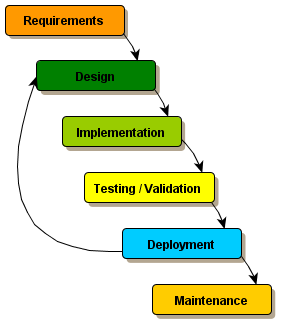
\includegraphics[scale=0.65]{pages/chapter3/figures/softwarecycle.png}
				\caption{Adapted Waterfall Model}
				\label{fig:AdaptedWaterfallModel}
			\end{figurehere}
			\vfill
			
		\end{multicols}	
		
		In the next section I will identify these requirements solidified, negating the requirement for change in the resulting development process. 
		\newline
	}
	
	
	\vspace{-3mm}
\section{Requirements}	

	\normalsize
	{		
		The elicitation of requirements can be obtained from many different techniques.
		The categorisation of requirements capture methods according to \citet{Goguen} can be divided into 4 main categories,
		traditional, cognitive, collaborative \& contextual techniques.	

		\vspace{-3mm}
		\begin{multicols}{2}
		
			\begin{itemize}
				\item \textbf{Traditional} 
					\newline
					including introspection, reading existing documents, analysing data,
					interviews, surveys \& questionnaires and meetings.
				\item \textbf{Cognitive}	
					\newline
					including task analysis, protocol analysis \& knowledge acquisition techniques.
		
		\vfill
		\columnbreak
		
				\item \textbf{Collaborative}	
					\newline
					including group techniques, workshops, prototyping \& participatory design.					
				\item \textbf{Contextual}	
					\newline
					including ethnographic analysis, discourse analysis \& sociotechnical methods.
					\newline
			\end{itemize}
		
		\end{multicols}	

		\textit{Those who have completed human computer interaction studies will be familiar with these techniques.
		These techniques are outside the scope of this report and I ask the reader to refer to Jakob Neilson 
		and his usability books series, which describe these techniques in detail.}
		\newline
		\newline
		Although no one categorisation was used in the elicitation of the requirements, there was a particular affinity
		to the cognitive category.  I, having previous experience in the role of Unix Systems Administrator in multi nationals corporations,
		identified with the repetitive processes in place in these companies. The tasks, protocol compliance and knowledge acquisition  
		incepted the concept and the key requirements of this project.  The following marchitecture (or marketecture) presents the key requirement artefacts.		
	}
	
	\vspace{3mm}
	\noindent\begin{minipage}{\textwidth}
			
		\begin{figurehere}
			\centering
			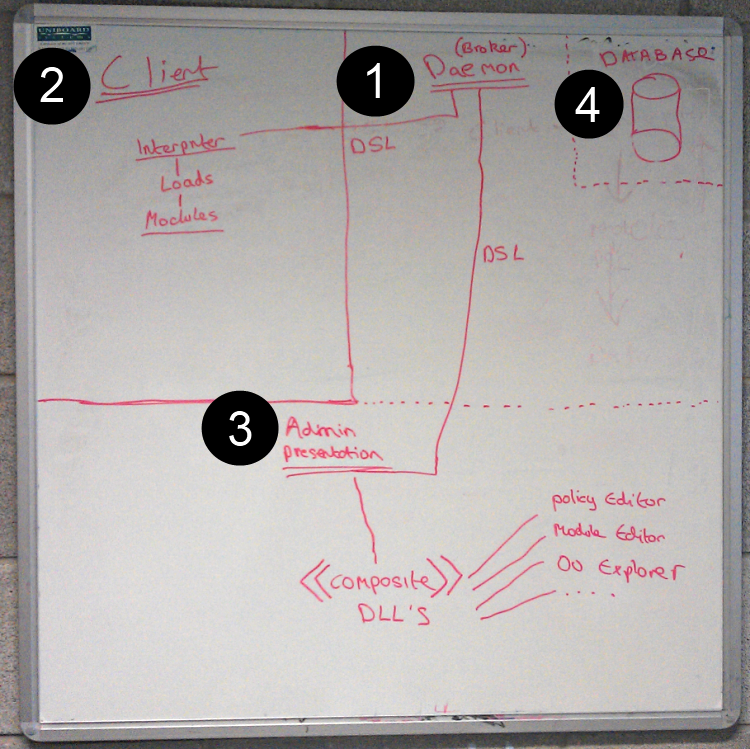
\includegraphics[scale=0.45]{pages/chapter3/figures/march2.png}
			\vspace{-2mm}
			\caption{Marchitecture}
			\label{fig:Marchiteture}
		\end{figurehere}	
	
	\end{minipage}	
		
	\vspace{3mm}
	\normalsize
	{
		To begin to understand the requirements and the resulting implementation,  Fig. \ref{fig:Marchiteture} 
		presents a marchitecture of a high level architectural design.  
		The marchitecture indicates the four main artefacts that support the requirements.
		
		\vspace{-3mm}
		\begin{multicols}{2}
		
			\begin{enumerate}[itemsep=0pt,parsep=0pt]

				\item \textbf{Daemon (Broker - Server)} 
					\begin{itemize}
						\item Broker between the admin presentation and the clients 
					\end{itemize}	
					
				\item \textbf{Client} 
					\begin{itemize}
						\item Interpreter which parses the domain specific language (DSL)
						\item Interpreter which loads modules to extend the parsing (rules) capabilities of the interpreter.
					\end{itemize}

			\columnbreak
					
				\item \textbf{Admin Presentation}	
					\begin{itemize}
						\item Linux Group Policy Administrator interface 
						\item Composite architecture
						\item Creates rules in the form of a domain specific language (DSL)
					\end{itemize}	
					
				\item \textbf{Database} 
					\begin{itemize}
						\item Ultimately stores all domain specific data
						\item Policies ( domain specific language )
					\end{itemize}	
					
			\end{enumerate}		
			
		\end{multicols}
		\vspace{-1mm}
		
		A recurring artefact here is the domain specific language (DSL). So I will provide a fifth section
		
		\begin{enumerate}
			\setcounter{enumi}{4}
			\item \textbf{Domain Specific Language (DSL)} 
				\vspace{-2mm}
				\begin{itemize}
					\item How rules are specified through a domain specific language
				\end{itemize}			
		\end{enumerate}		
	}		
	
	
	\section{Architecture}
	
	In the words of Martin Fowler, ``The software industry delights in taking words and stretching them into a myriad of subtly contradictory meanings,
	one of the biggest suffers is architecture'' - \citet{FowlerPatternsArchiteture}.  
	This is the perfect quote to describe the problem of defining what software architecture is.  
	The reader, you, has just read that line, interpret it and took your own profound meaning from it.  
	This a similar to the scenario of identifying what is deemed to be structurally relevant in a software product.  
	From a high level perspective most people can identify the main structural components of a software product, 
	however as the analysis continues, disagreement lurks, and the resulting definition gets blurred.
	\newline
	\newline
	As architecture is an inherited word from the construction industry, I'm going to go back to the earliest written works on the definition of
	architecture.  De Architectura by the roman architect Vitruvius, said architecture should satisfy three main principles, firmitas, utilitas, venustas,
	or durability, utility and beauty.
	\newline
	\newline
	Dan  known as ``the father of the spreadsheet'' wrote a paper, ``software that last 200 years'', says that we need to start thinking
	about software in a way that mimics the construction of bridges, dams and sewers.  Since software has only been around for a fraction of this time
	it's hard to determine whether the practices currently employed in software construction are going to stand the test of time.  
	There is still Fortran code(1956) running today as well as Lisp(1958); however, the only product still running and constantly being evolved is Unix(1959).
	Dan Bricklin makes the argument, a software's durability is a product of its marketing strategy and that bridges would not be very successful 
	if we tore it down every 10 years.  Unix and its derivatives are successful, along with the GNU (Gnus Not Unix) utils, e.g Emacs 1978. 
	\newline
	\newline
	This brings us to utility, if Unix were not useful, it and its derivatives would have died out long ago.  Its usefulness, in all manner of products
	from embedded systems to desktop personal computers and mainframes has been proven.  Vitruvius says that it should be useful and provide function to the people 
	using it.
	Beauty, the final principle of architecture according to Vitruvius is concept that changes with culture and time.  The austerity of time proven techniques
	compared to new paradigms, new design patterns, and the concept of beautiful software architecture seems to change like the weather.
	\newline
	\newline
	To satisfy the reader I will finish up with a definition of software architecture according to the most successfully marketed software developers
	Microsoft, \textit{``Software application architecture is the process of defining a structured solution that meets all the technical requirements,
	while optimising common quality attributes such as performance, security and manageability''}

	\subsection{Software Architecture}		
	
	There are many influencing software solutions that have influenced my thinking on software architectures and how they are deemed successful,
	but primarily useful to me and the end users.  Software that exhibits modular or pluggable characteristics allows for a richer user experience.
	Therefore the development of a software product that exhibited these characteristics was a primary concern.  
	Such frameworks as JQuery for Javascript, .Net for rapid application development and CodeIgnitor for PHP have 
	significantly influenced me.  So much that I no longer look to reinvent the wheel but try in most scenarios to avail of mature already 
	established frameworks to create software.
	\newline
	
		
	\vspace{-2mm}
\section{Daemon - (Broker - Server)} 

	\normalsize
	{
		The preferred name for a ``server'' in the Linux domain is ``daemon''.  The concept of a ``daemon'' is not unlike the concept of a ``server'',
		however using the term ``daemon'' negates the ambiguity associated with a ``server process'' running on a ``server computer''.  
		Throughout this section the term ``daemon'' will be used in regards to the process and the term 'server' will be used in reference to a 
		``daemon'' running on a server computer.  
		\newline
		\newline
		Furthermore the term ``broker'' creates yet more ambiguity, in that it is associated with an architectural pattern for the message validation, 
		transformation and routing.  For the sake of simplicity the term ``broker'' will be used to convey the facilitated communication 
		amongst peer processes, where a ``daemon'' in the middle between two computers facilitates this, effectively decoupling them from one another.
	}

	\vspace{3mm}
	\subsection{Requirements}
	
		\vspace{-5mm}
		\begin{multicols}{2}
		
			\begin{enumerate}[itemsep=1pt,parsep=1pt]
				\item 	Support for multiple clients			 
				\item 	Use of PERL  
				\item 	Scalable to handle 100's of clients
			\columnbreak
				\item   Master with multiple slave servers. 			
				\item   Push \& Pull technologies
			\end{enumerate}
			
		\end{multicols}
		
	\subsection{Technologies}
	
		\vspace{-5mm}
		\begin{multicols}{2}
		
			\begin{itemize}
			
				\item \textbf{PERL threads}	
					\newline								
					PERL threads were used extensively in the application for the client server model to gain maximum performance.  
				
				\item \textbf{PERL threads::shared}	
					\newline								
					To shared variables amongst threads.
										
				\item \textbf{PERL Thread::queue}	
					\newline								
					Queues were used extensively in both the client and the server.  The server has an incoming queue,
					processing queue and an outgoing queue.  The queues are thread safe and are first come first served basis
					ensuring ordered processing.
							
				\item \textbf{PERL Thread::Semaphore}	
					\newline								
					Certain critical sections in the client and server where identified and errors avoided by using semaphores.
					
		\columnbreak			
					
				\item \textbf{PERL IO::Socket}	
					\newline								
					A low level socket implementation was preferred for maximum performance.				
					
				\item \textbf{PERL POSIX}	
					\newline								
					Portable Operating System Interface (POSIX) was used in the application for the signalling of 
					threads and user interrupts which is a small subset of the POSIX API.  
					
				\item \textbf{PERL JSON}	
					\newline								
					For message passing in the implementation between the nodes this was the preferably choice for message passing.
						
				\item \textbf{PERL Sys::Syslog}		
					\newline							
					Syslog the de-facto means of logging in Linux and as such the choice to use Sys::Syslog 
					to log client - server interactions was required.
					
				\item \textbf{PERL DBI}			
					\newline						
					This database abstraction layer decouples the programmer from specific database API.   As it is a wrapper
					a common database connection string is used to specify the database type and the abstraction layer takes care of the specific
					API calls.  As such this allows for the use of most common database technologies, such as hierarchical, relation and object 
					oriented databases.
					
			\end{itemize}	
			
		\end{multicols}
	
	\subsection{Design}
			
		\normalsize
		{
			Although not subscribing to any particular design when designing the client server architecture,
			there were multiple influencing sources that lead to the architecture shown in Fig. \ref{fig:ServerQueues}.
			The book \textit{Pattern Oriented Software Architecture - Patterns for concurrent and networking objects} was a key 				
			influence on this simplified design, specifically with reference to the key aspects of the ``interceptor'' and ``leader / followers''
			design patterns.
			
			\noindent\begin{minipage}{\textwidth}
			
				\begin{figurehere}
					\centering
					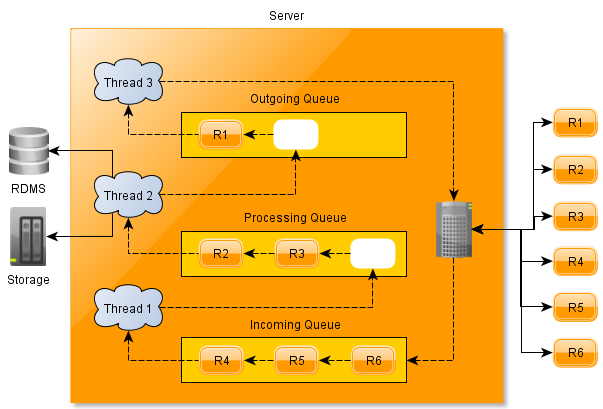
\includegraphics[scale=0.7]{pages/chapter3/figures/server-marchitecture.png}
					\caption{Server Queues}
					\label{fig:ServerQueues}
				\end{figurehere}	
			
			\end{minipage}
			
			\vspace{5mm}
			The architecture presented shows (R)equests moving through the internal data lanes of the implementation.
			Three queues are the main transition points within the architecture, namely the incoming, processing and 
			outgoing queues and the associated threads 1, 2 \& 3.  
			These requests internal messages can be divided into two major categories, Administrator and Client requests.
						
			\vspace{-3mm}
			\begin{multicols}{2}	
			
				\begin{itemize}[itemsep=1pt,parsep=1pt]
					\item \textbf{Administrator Requests}
						\begin{itemize}
							\item Module List
							\item Save / Update Module
							\item Synchronise Policies
							\item Push Policies to clients 
							\item Push Modules to clients
						\end{itemize}
				
				\columnbreak
						
					\item \textbf{Client Requests}
						\begin{itemize}
							\item Module Update
							\item Policy Update
						\end{itemize}					
				\end{itemize}	
				
			\end{multicols}	
			
			Although not immediately indicated the requests are asynchronous, meaning that the connection to the client
			is dropped as soon as the request is accepted.  By analysing the diagram we can also see that the queues enforce 
			the ordering of the events and subsequent resource interaction, such as database access or disk access.
			\newline
			\newline				
			The incoming queue is important as requests must be handled as fast as possible when implementing a server.
			If too many connections to a socket are open (IP address bound to a port eg. 127.0.0.1:80) there is the
			possibility of the server reaching the maximum allowed by the operating system.  This in turn this would give a busy
			signal to the subsequent clients trying to connect.  Connections that are accepted are immediately inspected
			for its request and this request is put into the incoming queue.  Finally thread 1 is responsible for determining
			whether the messages is well formed before being placed into the processing queue.				
			\newline
			\newline
			The processing queue is the next main transition for a request. In the processing queue the requests internal 
			message is analysed by thread 2 and subsequent processing is done depending on the request.  
			Once the processing is complete the request is put into the out going queue.	
			\newline					
			\newline
			Finally Thread 3 and the associated outgoing queue is responsible for sending a response back to the client/administrator 
			where applicable.  It is worth point out at this stage that the envelope in which the request is encapsulated, 
			holds information such as the peer IP address, peer port, peer request etc.
			\newline
			\newline
			With this information and the daemon response inserted into the request envelope by thread 2, 
			the outgoing queue is then processed by thread 3.  Thread 3 opens a connection to the destination and sends the response
			to the requester.					
		}				

	\vspace{4mm}
	\subsection{Architecture}
		\label{sec:serverarch}
		
		\normalsize
		{
			An introduction to software architecture by \citet{introsoftwarearchitecture} makes reference to state transitions 
			as an important aspect of the architectural design.  Fig. \ref{fig:ServerQueues} on the previous page
			offers three primary state transitions.  
			
			\vspace{-5mm}
			\begin{multicols}{3}
			
				\begin{itemize}[itemsep=1pt,parsep=1pt]
					\item \textbf{Incoming}				
					\item \textbf{Processing}		
					\item \textbf{Outgoing}	
				\end{itemize}	

			\end{multicols}		

			As a request passes through these data lanes or queues, the action of moving from one state to another
			offers pre marshalling and post marshalling capabilities.  We can extend the transitions as follows :
			
			\vspace{-2mm}
			\begin{multicols}{3}
			
				\begin{itemize}[itemsep=1pt,parsep=1pt]
				
					\item Incoming	
						\begin{itemize}
							\item \textbf{Pre incoming}				
							\item \textbf{Post incoming}	
						\end{itemize}
						
						
					\item Processing	
						\begin{itemize}
							\item \textbf{Pre processing}				
							\item \textbf{Post processing}	
						\end{itemize}
						
					\item Outgoing	
						\begin{itemize}
							\item \textbf{Pre outgoing}				
							\item \textbf{Post outgoing}	
						\end{itemize}
						
				\end{itemize}
				
			\end{multicols}				
		
			Each of these states offers transition points and the ability to include extensions to the framework
			to target specific requirements.  As an example of this, the implementation of the architecture allows for the addition
			of different security extensions for the both the pre incoming and pre outgoing transitions.
			In an example scenario an encrypted request that has been accepted into the incoming queue must first be decrypted
			before processing of the encrypted data can be accomplished.  Similarly the encryption of the outgoing response
			can be handled at the pre outgoing transition.  The following eight steps presented can be are identified in Fig. \ref{fig:Transitionstatesmarshalling}.
			\newline
			
			\begin{enumerate}[itemsep=1pt,parsep=1pt]
				
				\item Encrypted peer request is received			
				\item Request is added to the incoming queue	
				\item Thread 1 processes next request on the incoming queue
				\item Encryption extension decrypts message \textbf{(pre marshalling)}
				\item Thread 1 places decrypted request into processing queue \textbf{(post marshalling)}
				\item Thread 3 processes next item on out going queue
				\item Encryption takes place on the out going message \textbf{(pre marshalling)}
				\item Thread 3 sends the message to the peer \textbf{(post marshalling)}
				
			\end{enumerate}
					
			\vspace{4mm}
			This concept of pre and post marshalling effectively allows for the integration of different extensions to cover a multitude of
			future requirements and upgrades. These extensions could provide concepts such as load balancing, priority queues,
			multi-threaded queues and integration with other directory service systems.  
			\newline
			\newline
			Due to the time constraints of the project the decision to implement the daemon in this fashion provides the ability
			to satisfy the requirement of a master slave paradigm.  In an example scenario, the master server could provide load balancing
			by re routing incoming requests to slave daemons running on other servers. The potential resource heavy and time sensitive processing operation
			is then passed and balanced among these slave servers.  
			\newline
			
			\vspace{-3mm}
			\noindent\begin{minipage}{\textwidth}
				
				\begin{figurehere}
					\centering
					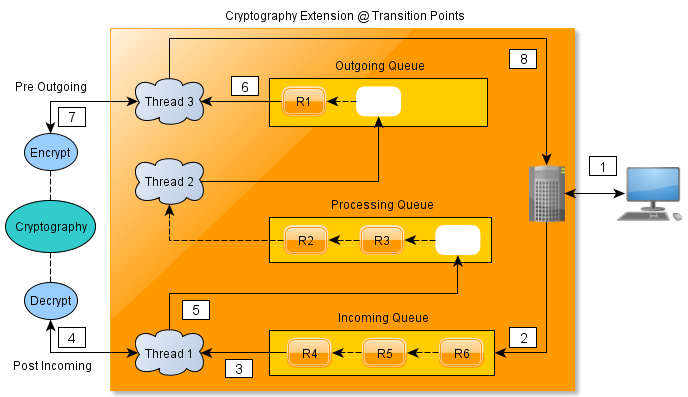
\includegraphics[scale=0.65]{pages/chapter3/figures/servertranitionstates.png}
					\caption{Transition states marshalling}
					\label{fig:Transitionstatesmarshalling}
				\end{figurehere}	
			
			\end{minipage}
		}
		

\newpage
		
	\subsection{Coding} 		
	
		\normalsize
		{
			The discussion of the design and architecture covers the following five technologies. These cover the basic concepts of threading and critical sections, first in first out (FIFO) queueing data structures
			and key concepts of socket programming. 
		}			
		
		\begin{itemize}[itemsep=1pt,parsep=1pt]
			\item \textbf{PERL threads}					
			\item \textbf{PERL threads::shared}				
			\item \textbf{PERL Thread::queue}	
			\item \textbf{PERL Thread::Semaphore}				
			\item \textbf{PERL IO::Socket}			
		\end{itemize}
			
					
		\normalsize
		{
			All of these topics are huge topics in themselves and are well understood fundamentals in computer science.  
			Therefore in this section I'm going to cover the more opaque technologies and provide coding snippets
			to support the reasoning for the choice of these technologies.
			\newline
		} 
		
			\begin{itemize}[itemsep=1pt,parsep=1pt]
				\item \textbf{PERL POSIX}						
				\item \textbf{PERL JSON}	
				\item \textbf{PERL Sys::Syslog}							
				\item \textbf{PERL DBI}							
			\end{itemize}
			
		\vspace{3mm}
		\large{\bfseries{POSIX}}
		
		\normalsize
		{
			The Portable Operating System Interface (POSIX) is an application programmers interface for maintainability compatibility between operating systems.  
			The use of POSIX in the implementation was primarily used for thread signalling and ensuring the clean shut down of the daemon.  
			\newline
			\newline
			In order to communicate with the daemon from an administration point of view
			where an administrator is logged onto the server some sort of inter-process communication is required.  For example, 
			rather than abruptly killing the server daemon with a ``kill -9 daemon'' command, named pipes were
			used to send this messages to the daemon.
			\newline
			\newline
			Named pipes are a basic form of inter process communication in Unix, Linux, Windows and Mac operating systems, however the semantics and resulting implementations differ.
			In Unix the implementation of this concept is achieved via use of the file system.  
			\newline
			\newline
			The mkfifo command on Unix and derivative platforms, makes use of the POSIX API to signal the kernel to
			prepare a file on the file system that acts as a first in first out queue, for inter process communication.  Piping information into this file is placed in shared memory. 
			The receiving process can then read this file (effectively the memory) achieving inter process communication.
			An example of this is given in Fig \ref{fig:perlreatepipe}.
		}
		
\newpage
						
		\begin{figurehere}
			\inputminted[linenos=true,fontsize=\footnotesize,tabsize=2]{perl}{pages/chapter3/smippets/perlfifo.pl}
			\vspace{-2mm}
			\caption{Creating and reading a named pipe}
			\label{fig:perlreatepipe}
		\end{figurehere}
		
		\vspace{5mm}
		\normalsize
		{
			In this example a named pipe is created and then opened for reading and writing.  As soon as data is piped into the file, this line is read using the chomp Perl function.
			The line is inspected for keywords, in this case ``stop'' and the internal variable ``continue'' is set to minus one.  All other threads within the application
			implement looping constructs based upon this ``continue'' variable.  When ``continue'' it is set to minus one,  this loop constructs discontinue, illustrated by the coding snippet in Fig. \ref{fig:perlqueues}.
		} 
				
		\begin{figurehere}
			\inputminted[linenos=true,fontsize=\footnotesize,tabsize=2]{perl}{pages/chapter3/smippets/threadscont.pl}
			\vspace{-2mm}
			\caption{Threads discontinue processing}
			\label{fig:perlqueues}
		\end{figurehere}
		
		\vspace{4mm}
		\normalsize
		{
			The second use of signalling is for the scenario where interrupts such as a kill signal is sent to the daemon process.
			As an example I will provide a simple scenario of running the daemon in the shell console context. Typically when a daemon is launched from within
			the context of a shell it detaches itself from the console.  However if it does not do this, when the shell is finished or is closed 
			it kills any processes which it has launched.  This concept is familiar to programmers
			who write managed code where the garbage collector removes unused or unreferenced artefacts in memory.
			\newline
			\newline
			Running a daemon in the shell context present a problem.  Cleanly shutting down the process is important when the cancel or kill signal is fired.
			This is typically done on systems using ``CTRL \textasciicircum  C''.  To ensure clean shut down and the termination of threads, this signal must be ``caught''.
			Threads must be told to shut down and finally terminate the program.
			\newline
			\newline
			This is accomplished via POSIX,  terminals typically implement POSIX and encompassing signalling.  So when ``CTRL \textasciicircum  C'' is 
			pressed the terminal catches the signal and terminates the application.  Therefore we must intercept this signal and handle this terminal event.  
			PERL provides POSIX support and with this we can intercept the kill signal;  Fig. \ref{fig:perlsignals} presents this.
			\newline
		} 
		
		\begin{figurehere}
			\inputminted[linenos=true,fontsize=\footnotesize,tabsize=2]{perl}{pages/chapter3/smippets/signals.pl}
			\vspace{-5mm}
			\caption{PERL Signals}
			\label{fig:perlsignals}
		\end{figurehere}
		
		\vspace{3mm}		
		\normalsize
		{
			In this example ``SIG'' which is a global variable provided by the POSIX module in PERL provides a means to map a signal to a closure
			or method stub.  When the ``INT'' signal is received the ``signal\_interrupt'' is called which tells the server to shut down.  
			In order to override repeated ``CTRL \textasciicircum  C'' events we re-map the INT signal once again to the ``signal\_interrupt'' closure.
			Finally the client sleeps for 1 second, this typically will allow threads to shut down before the application terminates.
			\newline
			\newline
			Context switches in the kernel are guaranteed to be no more than 500ms. This duration allows all attached threads
			to shut down or terminate before the application exits.  Typically in a modern processor, context switches can occur up
			20,000 times per second. This means that this amount of threads could be terminated in this time allotment. In the implementation
			the stop method in the daemon class has more than enough time to achieve this goal.  An excerpt of this stop method is provided in Fig. \ref{fig:StopServerThreads}.
		} 
		
		\vspace{2mm}
		\begin{figurehere}
			\inputminted[linenos=true,fontsize=\footnotesize,tabsize=2]{perl}{pages/chapter3/smippets/serverstop.pl}
			\vspace{-4mm}
			\caption{Stop Server Threads}
			\label{fig:StopServerThreads}
		\end{figurehere}
		
\newpage

		\large{\bfseries{JSON}}	
		
		\normalsize
		{		
			Javascript Object Notation (JSON) is a lightweight data-interchange format for the transfer of platform independent communication.  
			The name may suggest that it is for Javascript only, however most of the 3rd and 4th generation programming languages implement JSON parsers.  
			The choice of JSON over the typically used Extensible Markup Language(XML) was the syntactic verbosity factor.  There are examples on json.org that indicate
			XML can be 300\% more verbose than JSON.  In a system that is dependent on speed and efficiency, the smaller and hastily parsing of messages is important.
			Therefore JSON was a good candidate for encapsulation of messages due to its' lightweight envelope.  Initially I had devised my own short form syntax for messages
			however as the implementation grew and the message became more complex, the need for a better envelope and formatting of messages was required.
		}
		
		\vspace{2mm}
		\begin{figurehere}
			\inputminted[linenos=true,fontsize=\footnotesize,tabsize=2]{perl}{pages/chapter3/smippets/jsonmessage.pl}
			\vspace{-2mm}
			\caption{JSON Client Request}
			\label{fig:ClientJsonRequest}
		\end{figurehere}
				
		\normalsize
		{	
			In section \ref{sec:serverarch} identified the messages that the server dealt with, one of them being a client update.  
			As an example Fig \ref{fig:ClientJsonRequest} presents a request from a client for a policy update.  The key ``request'' holds the value
			or the intended request to be sent to the server.
			\newline
		}
		
		\large{\bfseries{Syslog}}	
		
		\normalsize
		{		
			Syslog is a data logging standard used by Unix and derivatives as a means to decouple processes from operating system logging mechanism.
			These logs can then be checked by administrators of the environment and reports made from them.  In order to debug daemons where the standard output is not visible
			as the daemon is not attached to a console, a means of logging messages is required.  The integration with the system implementation logging features
			is expected and as such the choice for Syslog was mandatory.
			\newline
			\newline
			An entry is made into the Syslog configuration.  The entry is then used to create a pipe by Syslog to which process can redirect messages to; 
			 resulting in the corresponding file.
			\newline
			\begin{center}
			local6.*						/var/log/lgp
			\end{center}
			\vspace{5mm}
			The following PERL excerpt in Fig. \ref{fig:PerlSyslog} shows the use of this logging mechanism and the corresponding log file excerpt below it.
		}
				
		\begin{figurehere}
			\inputminted[linenos=true,fontsize=\footnotesize,tabsize=2]{perl}{pages/chapter3/smippets/syslog.pl}
			\vspace{-2mm}
			\caption{PERL Syslog}
			\label{fig:PerlSyslog}
		\end{figurehere}
		
		\vspace{5mm}
		\normalsize
		{
			Mar 29 17:16:25 testmachine2 cmain.pl[3657]: Client created tcp connection on 192.168.1.10:50000
			\newline
		}
						
		\large{\bfseries{DBI}}	
		
		\normalsize
		{					
			As the back end of the architecture depends on database for storage, a major concern is the subscription to a vendor specific database.
			This vendor database may in the future be deprecated and the need to migrate to a new database vendor may occur.
			The PERL DBI (PERL Database Interface) offers an abstraction for programmers using the PERL programming language from vendor specific
			database implement ion application programmer interfaces.  Programmers who are familiar with connection strings such as that used in .NET of ODBC will be 
			familiar with this concept.  Other languages such as PHP provide the PHP Data Objects (PDO) as a comparable abstraction.  
			This abstraction layer allows for the choice of database based upon a connection string.
			In Fig. \ref{fig:Perldbi} the connect stub of the database PERL module in the implementation provides the ability to change the database type
			at rune time.
		}
		
		\vspace{2mm}
		\begin{figurehere}
			\inputminted[linenos=true,fontsize=\footnotesize,tabsize=2]{perl}{pages/chapter3/smippets/dbi.pl}
			\vspace{-2mm}
			\caption{PERL DBI}
			\label{fig:Perldbi}
		\end{figurehere}	 
		
\newpage
	
	\subsection{Analysis}
	
		\normalsize
		{					
			Many concerns arise when attempting to do an analysis of the daemon; namely speed, scalability, extensibility, maintainability, 
			portability and security.  There are many topics.  In this analysis I'm going to tackle the speed concerns, and the resulting scalability. 
			\newline
			\newline
			Stress testing was done on the implementation as a means to elicit empirical evidence to validate the requirements, namely
			``Scalable to handle 100's of clients''.  A stress test harness was setup to address this concern.  The stress test consisted of six virtual machines, 
			one server and five clients running on a single computer.	Table \ref{tab:TestMachine} presents the test machine characteristics.
			\newline
		}
		
		
		\begin{tablehere}	
		
			\begin{tabular}{rrrr}

				{\bf Test Machine} 						& {\bf Cores} 	& {\bf Threads} 		&            		\\ \hline
				{\bf Intel Core I7 965 @ 3.2 GHZ} 		&          4 	&          8 			&            		\\
														&            	&            			&            		\\
														&  {\bf Ram} 	&            			&            		\\ \hline
				{\bf DDR3 PC3-10666 Triple Channel } 	& 16 Gigabytes 	&            			&            		\\
														&            	&            			&            		\\
														& {\bf IOPS} 	& {\bf Form Factor} 	&  {\bf RPM} 		\\ \hline													
				{\bf OCZ RevoDrive } 					&      70000 	& PCI-Express RamDrive 	&        N/A 		\\
														&            	&            			&            		\\
				{\bf Vmware Virtual Machines} 			&  {\bf Ram} 	& {\bf Threads} 		& {\bf Function} 	\\ \hline
				{\bf Redhat 32} 						& 2 Gigabytes 	&          2 			&     Daemon 		\\
				{\bf Fedora 32} 						& 2 Gigabytes 	&          2 			&     Client 		\\
				{\bf Fedora 64} 						& 2 Gigabytes 	&          2 			&     Client		\\
				{\bf Gentoo} 							& 2 Gigabytes 	&          2 			&     Client 		\\
				{\bf Ubuntu} 							& 2 Gigabytes 	&          2 			&     Client 		\\
				{\bf Open Suse} 						& 2 Gigabytes 	&          2 			&     Client 		\\

			\end{tabular}  
			
			\caption{Test Machine}
			\label{tab:TestMachine}
			
		\end{tablehere}	
		
		\vspace{5mm}
		\normalsize
		{					
			It was important to negate all possible bottle necks in the test equipment.  To achieve characteristics of 
			enterprise level server performance. I negated the hard drive bottle neck that would be associated with personal computers.
			As in an enterprise environment, ``filers'' would be used as a data centres backbone for storage; due to their high performance.
			\newline
			\newline
			Making the comparison between OCZ RevoDrive in table \ref{tab:TestMachine} and that of consumer grade hard drive is presented
			in table \ref{tab:HardDrivesComparison}.  The form factor presented indicates approximately 14 times faster hard drive access speed.
			\newline
		}
		
		
		\begin{tablehere}	
		
			\begin{tabular}{rrrr}

				{\bf Comparison} 						& {\bf IOPS} 	& {\bf Form Factor} 	&  {\bf RPM} 		\\ \hline
				Sata 3 Hard Drive  						&        150 	& Sata 3 HDD 			&       7200 		\\
				Sata 3 Solid State Drive 				&       5000 	& Sata 3 SSD 			&        N/A 		\\

			\end{tabular}  
			
			\caption{Hard Drives Comparison}
			\label{tab:HardDrivesComparison}
			
		\end{tablehere}	
		
\newpage		
		
		\normalsize
		{					
			The test composed of 500 requests to the daemon to push out updates to the clients, each with a delay of 30ms between each request. 
			In effect this meant that there were 500 + (5 * 500) equalling 3000 asynchronous requests.
			\newline
			\newline
			A sampling interval of 1 second was used to capture information, such as processor, queueing and network loads.
			The resulting data is shown in Fig. \ref{fig:ServerCpuUsage}, \ref{fig:ServerQueueUsage} and \ref{fig:ServerNetworkUsage} respectively.
			\newline
		}		
		
		\noindent\begin{minipage}{\textwidth}
			
			\begin{figurehere}
				\centering
				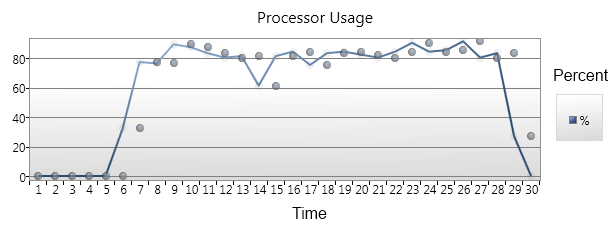
\includegraphics[scale=0.9]{pages/chapter3/figures/server-cpu.png}
				\vspace{-2mm}
				\caption{Server CPU Usage}
				\label{fig:ServerCpuUsage}
			\end{figurehere}	
		
		\end{minipage}
		
		\vspace{6mm}
		\noindent\begin{minipage}{\textwidth}
			
			\begin{figurehere}
				\centering
				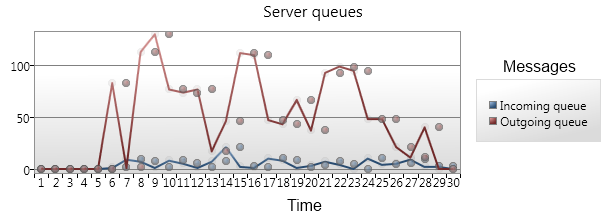
\includegraphics[scale=0.9]{pages/chapter3/figures/server-queues.png}
				\vspace{-2mm}
				\caption{Server Queues Usage}
				\label{fig:ServerQueueUsage}
			\end{figurehere}	
		
		\end{minipage}
		
		\vspace{6mm}
		\noindent\begin{minipage}{\textwidth}
			
			\begin{figurehere}
				\centering
				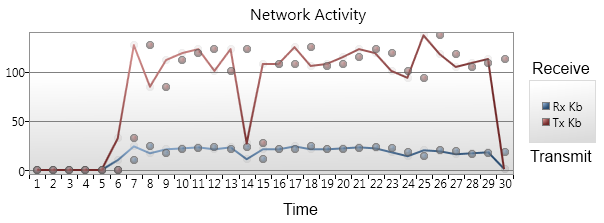
\includegraphics[scale=0.9]{pages/chapter3/figures/server-network.png}
				\vspace{-2mm}
				\caption{Server Network Usage}
				\label{fig:ServerNetworkUsage}
			\end{figurehere}	
		
		\end{minipage}
			
		\vspace{5mm}
		\normalsize
		{					
			The test took approximately twenty five seconds, equaling one hundred client updates per second.  In the implementation however,
			the client checks for updates every twenty minutes.  As there is 1200 seconds in this time, potentially under 
			optimal conditions the server could handle 120,000 clients.  This hypothetical scenario is based upon a policy
			that equates to approximately one kilobyte and optimal testing conditions.  
			Under real conditions this scenario may not be feasible, due to larger policies and possible network degradation. 
			The achievement of 5\% of this performance this still equates to approximately six thousand client updates, in this twenty minute interval.		
			\newline
		}	
			
	
	\subsection{Improvements}

		\normalsize
		{					
			In \textit{Patterns of Enterprise Application Architecture} by Martin Fowler, he makes numerous references to case studies were 
			performance testing presented bottle necks in string processing.  The resulting degraded application performance was in some cases
			diabolical and light weight changes resulted in 100\% increased efficiency.  
			In the server architecture the daemon makes use of numerous text conditionals and JSON.  Ultimately these text conditionals need to be
			lexicographically parsed, resulting in high processor usage as indicated by figure \ref{fig:ServerCpuUsage}.
			\newline			
			\newline
			To begin to target this contention in future improvements, the use of JSON as an envelope for message passing might be dropped.
			Initially during development I did not use JSON, however as the complexity grew a need for a structured message was required, as sequenced
			events became difficult to maintain.
			\newline
			\newline
			Furthermore as the client sends requests as text, these text conditionals need to be lexicographically inspected and compared
			by the daemon to create the correct response.  These text conditionals could be replaced by integer values
			that require very little computation in terms of comparison by a processors arithmetic logic unit (ALU).  
			\newline
		}	

	
	
	
	
	
	
	
	
	
	
	
	
	
	
	


\section{Client} 

	\normalsize
	{
		In this section the discussion of the client; it's operations and supporting technologies will be consummated.
		along with a brief introduction to the transliteration of the domain specific language.
		\newline
		\newline
		The client implementation is responsible for downloading a policy from the daemon and executing it.
		The execution of the policy, a domain specific language (DSL) is the application of the rules defined by the administrator.
		The client determines the operating system distribution it is executing on and through the use of an interpreter, it applies the policy  
		via distribution specific commands.  
	}

	\vspace{3mm}

	\subsection{Requirements}
	
		\begin{enumerate}[itemsep=1pt,parsep=1pt]
		
			\item 	Support for multiple distributions
			\item 	Client must be extensible
			\item 	Use of PERL 
			\item 	Updates to varying architectures
			\item   Push \& Pull technologies
			
		\end{enumerate}
		
	\subsection{Technologies}
	
		\vspace{-5mm}
		\begin{multicols}{2}
			
			\begin{itemize}
			
				\item \textbf{PERL threads}	
					\newline								
					PERL threads were used extensively in the application for the client server model to gain maximum performance.  
				
				\item \textbf{PERL threads::shared}	
					\newline								
					To shared variables amongst threads.
					
				\item \textbf{PERL Thread::queue}	
					\newline								
					Queues were used extensively in both the client and the server.  The server has an incoming queue,
					processing queue and an outgoing queue.  The queues are thread safe and are first come first served basis
					ensuring ordered processing.
					
				\item \textbf{PERL Thread::Semaphore}	
					\newline								
					Certain critical sections in the client and server were identified and errors avoided by using semaphores.
					
				\item \textbf{PERL IO::Socket}	
					\newline								
					A low level socket implementation was preferred for maximum performance.				
					
				\item \textbf{PERL POSIX}	
					\newline								
					Portable Operating System Interface (POSIX) was used in the application for the signalling of 
					threads and user interrupts which is a small subset of the POSIX API.  
							
				\item \textbf{PERL JSON}	
					\newline								
					For message passing in the implementation between the nodes this was the preferably choice for message passing.
				
				\item \textbf{PERL Sys::Syslog}		
					\newline							
					Syslog the de facto means of logging in Linux is assumed by all major daemon installations
					and as such the choice to use Sys::Syslog to log client server interactions was required.
					
				\item \textbf{PERL Filter::Simple}	
					\newline								
					Source filtering or pre processing is an immensely powerful feature of PERL. 
					Effectively, it allows or provides the ability to create micro languages such as a DSL by
					preprocessing the input script translating it as necessary.
					
			\end{itemize}	
		
		\end{multicols}	
	
	\subsection{Design \& Architecture}
							
		\normalsize
		{
			The client operates in the same way as the server architecture shown in Fig. \ref{fig:ServerQueues} with the minor exceptions.
			The two main differences of the client are the messages and the operations done within the in the processing queue.
			The design analysis in this section will be therefore focused upon these operations and the encompassing interpreter.  
			As the interpreter facilitates the parsing of the domain specific language (DSL) resulting in distribution specific commands, 
			the resulting architectural design evolved to support the extensibility of this framework and the interpreter.
			Fig. \ref{fig:ClientInterpretor} presents a high level design overview. 
			\newline

			\noindent\begin{minipage}{\textwidth}

				\begin{figurehere}
				\centering
				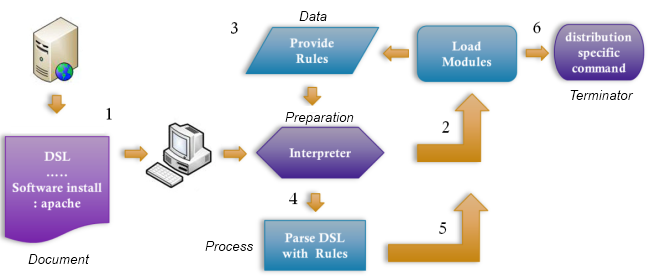
\includegraphics[scale=0.9]{pages/chapter3/figures/cleintmarchitecture.png}
				\caption{Client Interpreter}
				\label{fig:ClientInterpretor}
				\end{figurehere}	

			\end{minipage}
			
			\vspace{5mm}
			The marchitecture or control flow diagram (simplified) here presents the major sequences of events
			leading to a policy (set of rules) application.  A Unified Modelling Language (UML) Diagram is presented in 
			\ref{fig:InterpretorFramework} in Appendix 3.  
			
			\vspace{-3mm}
			\begin{multicols}{2}
			
				\begin{enumerate}
			
					\item \textbf{Receive policy update}	
						\newline								
						Server sends a policy update in the form of a domain specific language 
					
					\item \textbf{Interpreter initialises}	
						\newline								
						The interpreter is executed and loads the interpreter extensions (PERL modules)
						
					\item \textbf{Modules provide parsing rules}	
						\newline								
						The module(s) provide lexicographical parsing rules for the interpreter
						
					\item \textbf{Policy is parsed}	
						\newline								
						The interpreter parses the domain specific language (policy) using the parsing rules
						
				\columnbreak
						
					\item \textbf{lexicographically accepted lines are sent back to the modules}	
						\newline								
						For each successful line parsed, this line is sent back to the PERL module that provided the rule			
						
					\item \textbf{Module performs distribution specific command}	
						\newline								
						Further inspection is done on the line, eventually resulting in a distribution specific command				

				\end{enumerate}	
				
			\end{multicols}
		}		

		\normalsize
		{
			Unlike the server architecture, the messages can only come from the server to which the client is bound.
			There is no direct communication between the administrator interface and the clients, hence the concept of the broker.
			As an example, if the administrator sends  \textit{Push Policies} to the server, then the server iterates the known or 
			bound clients and pushes out the policy in the form of the DSL to the clients.
			\newline
			\newline				
			The client messages are as follows :
			
			\vspace{-3mm}
			\begin{multicols}{2}
			
				\begin{enumerate}[itemsep=1pt,parsep=1pt]
					\item \textbf{Request Policy Update}
					\item \textbf{Receive Policy Update}
					\item \textbf{Request Modules Update}
					\item \textbf{Receive Modules Update} 
				\end{enumerate}	
				
			\end{multicols}

			These messages provide a second point of interest from an administrator perspective.
			How does an administrator easily update the client and the interpreter modules?
			In a large enterprise environment updating the client with new modules via typical software installation
			means, ie. sitting at the computer and updating it, which is not feasible.  Any software extensibility provided by the client
			would be potentially negated by this time consuming operation.   Therefore the design to support extensibility
			has been bolstered by the ability to push out new client modules and updates. 
			\newline			
			\newline
			These modules are kept on the same server as the daemon.  The clients check for modules updates at set intervals.
			To reduce network traffic a checksum of each module is sent to the client. The client compares this checksum against it's local copy.
			If there is a difference, an update has occurred and this modified or new module is requested by the client from the daemon.
			\newline
			\newline
			This allows the administrators to create and modify modules on a continual basis, thereby meeting the enterprise specific 
			regulations and requirements, that can subject to change on a continual basis.
			\newline
		}		
	
	\subsection{Patterns}
	
		\normalsize
		{
			As previously discussed the modules have two primary functions :  
			
			\begin{itemize}[itemsep=1pt,parsep=1pt]
				\item \textbf{To extend the interpreter and the language that it understands }
				\item \textbf{The Interpretation of rules, resulting in distribution specific commands}
			\end{itemize}				
		}
			
			\vspace{-3mm}
			\begin{multicols}{2}
			
				Administrators who intend to implement new modules are implementing observers as seen in the Observer Design Pattern, Fig. \ref{fig:ObserverDesignPattern}.
				\newline
				\newline
				These observers provide new grammar to the interpreter, which in turn sends updates, using the Observer Design Pattern update mechanism. 
				Each individual rule(line) that is accepted by the interpreter using the provided grammar rules, is sent to all modules.	
				Each module knows if this update is detonated for it, as it has provided the rule to the interpreter.
			
				\columnbreak
				
				\begin{figurehere}
					\centering
					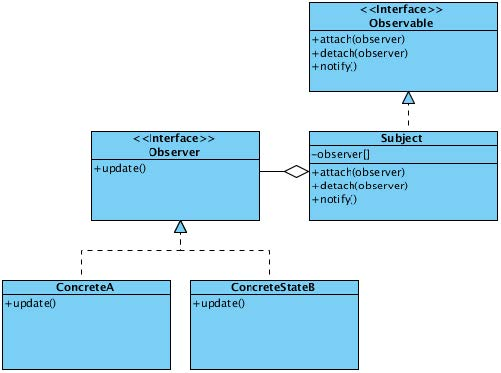
\includegraphics[scale=0.55]{pages/chapter3/figures/observer.jpg}
					\caption{Observer Design Pattern}
					\label{fig:ObserverDesignPattern}
				\end{figurehere}
			
			\end{multicols}
			
		\normalsize
		{			
			This offers the ability to provide modules outside of this preordained behaviour.  Modules could be designed to
			monitor, log or validate these messages and their outcomes.  This one to many relationship (policy line to modules) does create a 
			little extra processing, however, it provides more flexibility for administrators creating modules.  A module that has too many responsibilities
			may become difficult to maintain, therefore the separation of logging, monitoring \& validating into different modules are handled
			by this design decision.
			\newline
		}	
		
\newpage
	
	\subsection{Coding} 
	
		Dissecting the domain specific language (DSL) in Fig. \ref{fig:DSL},  we can see at the beginning the interpreter is included.  
		The interpreter which will eventually go on to read the DSL, firstly constructs the framework which in turns loads the modules.
		
		\vspace{4mm}
		\begin{figurehere}
			\inputminted[linenos=true,fontsize=\footnotesize,tabsize=2]{perl}{pages/chapter3/smippets/dsl}
			\vspace{-5mm}
			\caption{DSL}
			\label{fig:DSL}
		\end{figurehere}	
			
		\vspace{4mm}
		During the loading of the modules, the ``registerGrammer'' method is called on each module (Fig. \ref{fig:Loadmodules}).  
		There is pure assumption from module loader that module being loaded provides a new method and a ``registerGrammer'' method.
		This reflects the concept of late binding,  unlike the early binding method of using reflection to firstly inspect an object for a method
		and binding appropriately.
		
		\vspace{4mm}
		\begin{figurehere}
			\inputminted[linenos=true,fontsize=\footnotesize,tabsize=2]{perl}{pages/chapter3/smippets/loadmodules}
			\vspace{-5mm}
			\caption{Load modules - Simplified}
			\label{fig:Loadmodules}
		\end{figurehere}	
		
		\vspace{4mm}
		There are of course positive and negative effects of this.  As PERL has run time flexibility as seen in most interpreted languages.  
		Up front validation of the module implementation is difficult requiring a try and test approach of module development.  
		This would not be advisable in a live environment and should be done in a test harness,  a group of machines separate from the live environment.
		\newline
		The positive effect however, is that no compiling is required, and gives greater flexibility and interoperability in deployment of a 
		client onto an unknown system.
		\newline
		
		\large{\bfseries{Filter::Simple}}	
		
		\normalsize
		{					
			Syntax Directed Translation (SDT) of the domain specific language in Fig. \ref{fig:DSL} is achieved via source filtering.
			Syntax Directed Translation (SDT) is a method of translating sentential forms to machine code or some other 
			intermediary language, such as Java byte code.  There are many different techniques to achieve this outcome and 
			multiple operations may be done to the input before the translation is completed.  This is the fundamental process used by compilers 
			and interpreters.
			\newline
			\newline
			One of the initial steps in this process is the processing of preprocessor directives.
			Fig. \ref{fig:UseFilter} presents an example of the ``use'' keyword.  This tells the PERL interpreter that the module ``File2''
			will needed to be included, before any subsequent processing takes place.  The next stage of the interpretation, is in this example, 
			source filtering.	
			\newline
		}
		
		\begin{figurehere}
			\inputminted[linenos=true,fontsize=\footnotesize,tabsize=2]{perl}{pages/chapter3/smippets/usefilter.pl}
			\vspace{-5mm}
			\caption{File 1}
			\label{fig:UseFilter}
		\end{figurehere}
		
		\vspace{5mm}
		\normalsize
		{
			File 1 (Fig. \ref{fig:UseFilter}) provides the preprocessor directive ``use File2''.  File 1 (Fig. \ref{fig:UseFilter}) is then subject to source filtering.
			File 2 (Fig. \ref{fig:FilterSimple}) provides a filter block, which takes the input of the File 1 (Fig. \ref{fig:UseFilter}) and places it input the PERL
			variable \$\_.
			Grammar rules in the form of regular expressions, provided by the modules in Fig. \ref{fig:Loadmodules}, are then used to parse the data in the \$\_ variable.
			\newline
			\newline
			Delving further into this subject will take place in section \ref{sec:Domainspecificlanguage} (DSL).
			\newline
		}
		
		\begin{figurehere}
			\inputminted[linenos=true,fontsize=\footnotesize,tabsize=2]{perl}{pages/chapter3/smippets/filter.pl}
			\vspace{-5mm}
			\caption{File 2}
			\label{fig:FilterSimple}
		\end{figurehere}
		

	\vspace{4mm}
	\subsection{Analysis \& Improvements}
	
		The client solution developed meets the requirements imposed.  In the case for \textbf{support for multiple distributions} and \textbf{extensibility},
		Unix and derivatives provide PERL as standard.  The support for multiple distributions is then a matter of extensibility.
		This extensibility is achieved via the creation and modification of modules.  As new distributions are created and the distribution specific commands evolve 
		or change, this is ultimately handled by the extensibility nature of the interpreter via these modules.  
		\newline
		\newline
		As PERL is not a compiled language, updates can be pushed out to the clients regardless of the architecture.  
		In the future a test harness for the testing of modules should be provided.
		There is a risk of an administrator unintentionally distributing a fallible module, which could result in costly outcomes.
		\newline
		\newline
		Although the architecture presented meets the requirements, some improvements could be done to the interpreter.
		As the interpreter's grammar rules are provided in the form of regular expressions, the complexity of these rules
		could become rather difficult to understand.  However immensely powerful regular expressions are, for future improvement a relaxing of 
		this validation technique may be catered for.  Stubs or blocks that have opening and closing elements as seen in the extensible markup language,
		may provide the ability to break up parsing rules into more manageable discrete statements.
		\newline
	

	
	\section{Admin Presentation} 

	\subsection{Requirements}
	
		\begin{enumerate}[itemsep=1pt,parsep=1pt]
			\item Creating organisational units.
			\item Move objects in the organisational hierarchy.
			\item Hierarchy of organisational units.
			\item Modify policies.
			\item Rules creation results in DSL script.
			\item Provide means of importing rules.
			\item Push updates to the client.
		\end{enumerate}
		
	\subsection{Technologies}
			
		\begin{itemize}
			\item \textbf{C\#} 
				\newline
				C\# is a multi-paradigm programming language encompassing strong typing, imperative, 
				declarative, functional, generic, object-oriented, and component-oriented programming disciplines. [cit]
		
			\item \textbf{AvalonDock} 
				\newline				
				Avalondock is a windows presentation foundation(WPF) controls library that provides the 
				functionality of a dockable layout system for UserControls within a user interface.  It supports fly-out panes
				dockable pinning expanders and floating windows.				
		
			\item \textbf{AvalonEdit} 
				\newline						
				Avalonedit is the WPF rich text user control for editing source code in SharpDevelop the open source 
				alternative to Visual Studio.  The editor features many of the post Intellij integrated development environment features
				such as code completion, code folding and syntax highlighting.
				
			\item \textbf{Infralution localization} 
				\newline						
				Infralution localization is an open source class library that integrates localisation features easily into
				windows presentation foundation(WPF) projects by taking control of resources files associated with a visual studio project.  
				This middle tier layer between the compiled code and the translations provides a means to instantly change
				the language in an application at run time.
				
			\item \textbf{JSON.net}	
				\newline								
				Json.Net is an open source Javascript Object Notation framework for .Net.  
				For message passing in the implementation between the nodes this was the preferably choice for message passing.
				
			\item \textbf{Microsoft Prism Event Aggregator}	
				\newline								
				The Microsoft implementation of Marting Fowler's Event Aggregator was chosen as a means for internal message
				passing within the application framework as it allows for events to be decoupled for the publishers and subscribers.
				
			\item \textbf{Visual Studio 2010}		
				\newline							
				The Microsoft Visual Studio Integrated Development Environment is by far the best in the field for rapid application 
				development in my opinion.  The deployment options, such as Web/Desktop/Phone etc
				coupled with the Common Language Runtime (CLR) run time environment allows for the development of applications that bring interoperability and manageability
				to new heights.
				
			\item \textbf{Windows Presentation Foundation}	
				\newline								
				The Windows Presentation Foundation graphical subsystem introduced with .Net 3.0 and at the core of Windows Vista / 7 
				renders applications directly into DirectX and is graphically accelerated on industry standard graphics cards.  The 
				idea of desktop compositioning driven by earlier projects in the open source community such as Beryl and Compiz
				made the push for this.  Apple and Microsoft quickly followed suit.  Furthermore WPF provides a model view-view model 
				design approach for the separation of the code and interface design somewhat comparable to Model View Controller introduced
				by smalltalk.
				
			\item \textbf{Xaml}		
				\newline							
				The Extensible Application Markup Language (Xaml) is a declarative XML based language used for the creation of user interfaces.
				Xaml directly maps for CLR run time object instances and the attributes to the associated properties allowing for most of the
				user interface functionally to be kept out of the business model or controller.
				
		\end{itemize}			
		
	\subsection{Design}
	
		\normalsize
		{	
			The design of the Linux Group Policy presentation or administrator interface was extensive.  With up wards of fifty 
			thousand lines of code, the need for a high quality design was exigent.  The support for the 'ilities' or non functional requirements
			motivated the design and eventual architectural framework.   Many influences lead to the design of the composite framework, such authors 
			as Martin Fowler, Joshua Kerievsky and Gamma et al.
			\newline	
			\newline
			Fig. \ref{fig:designoverview} presents a high level architectural design model.
			The design could be described as a three tier architecture.  Where the separation of presentation, logic and the data is shown.
			This distinction however in reality a little clouded, but the three tier architecture seems the best method to articulate the real nature
			of the design.	
			\newline
			\newline			
		}

		\begin{figurehere}
			\begin{center}
			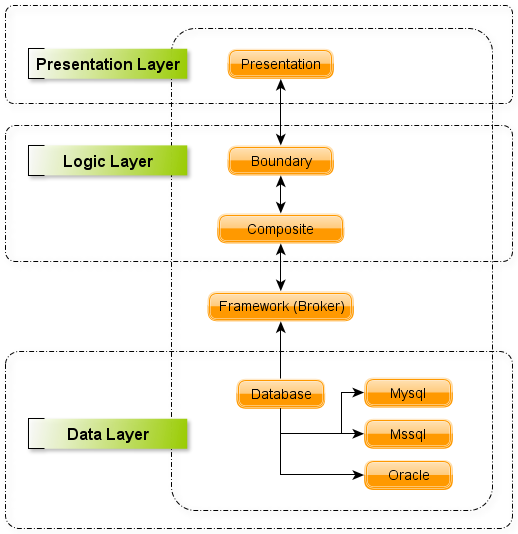
\includegraphics[scale=0.6]{pages/chapter3/figures/designarch.png}
			\end{center}
			\caption{Design Overview}
			\label{fig:designoverview}
		\end{figurehere}			

		\vspace{5mm}
		\normalsize
		{			
			Each composite has it's own responsibilities and encapsulates all the presentation and logic layers 
			for which it is concerned.  There are two composites that deviate from this assertion.
			\newline
			\newline
			It was decided upon to separate the data tier from the end composite developers.
			This separation of the data layer negates or reduces unfavourable database operations.
			The obfuscation of the structured query language(SQL) and the encapsulating of it into representing domain types provides traceability,
			monitoring and maintainability.
			\newline
			\newline
			The database composite is primarily concerned with the data layer, however it exhibits presentation (settings panes)
			and logic layer functionality also.  The database composite therefore abstracts all the domain concerns and the framework or the brokering layer 
			facilitates the access to this data layer or the database composite.
			\newline
			\newline
			The factory composite provides all the domain and architectural interfaces for the entire architecture.
			This framework layer decouples all composites and implements patterns to facilitate communication between these decoupled composites. 
			It does not provide a presentation or data layer, however it provides extensive logic layer functionality for the loading of the composites
			and subsequent brokered interactions.	
		}
		
\newpage
	
	\subsection{Architecture}		
				
		\vspace{-5mm}
		\begin{multicols}{2}
		
			The Architecture of the Linux Group Policy Studio Administration interface is comprised of separate interchangeable dynamic link libraries 
			as can be seen in the composite architectural overview in Fig. \ref{fig:archover}.  			
			This type of software technique is commonly known as composite or modular programming.  
			\newline
			\newline
			Each individual DLL (dynamic link library) is designed 
			for a specific scenario and encapsulates all the necessary logic for the scenario and its use cases.   
			This separation of concerns greatly improves the maintainability, reliability and reduces the fallibility of the software product as a whole.
			\newline
			\newline
			These dynamic link library components are loaded at run time and inspected via reflection for predefined architectural 
			interfaces.  Based on the interface the incorporation into the system is decided upon.  
			For example, if a class realises the interface IDatabaseStrategy,  we know this component is to be used by the Database connector 
			and therefore it is loaded and referenced in the appropriate location, making it accessible to the database connector.
			\newline
			\newline
			The main core of the modular framework consists of the lgp.components.factory dynamic link library which exposes the public static class 'Framework'.
			A static class is a class where all properties and methods are said to be static. C\# allows the use of the static keyword in the class definition
			thereby enforcing this rule. 
			\newline
			\newline
			Framework is a boundary class and with the use of the architectural and domain interfaces, it exposes the 
			dynamic link libraries concrete types that match, support, realise these interfaces.
			For example, rather that exposing the concrete Type 'Utilities' which is part of the framework;
			rather the interface for this type is exposed.  
		
			\columnbreak
		
			\begin{figurehere}
				\centering
				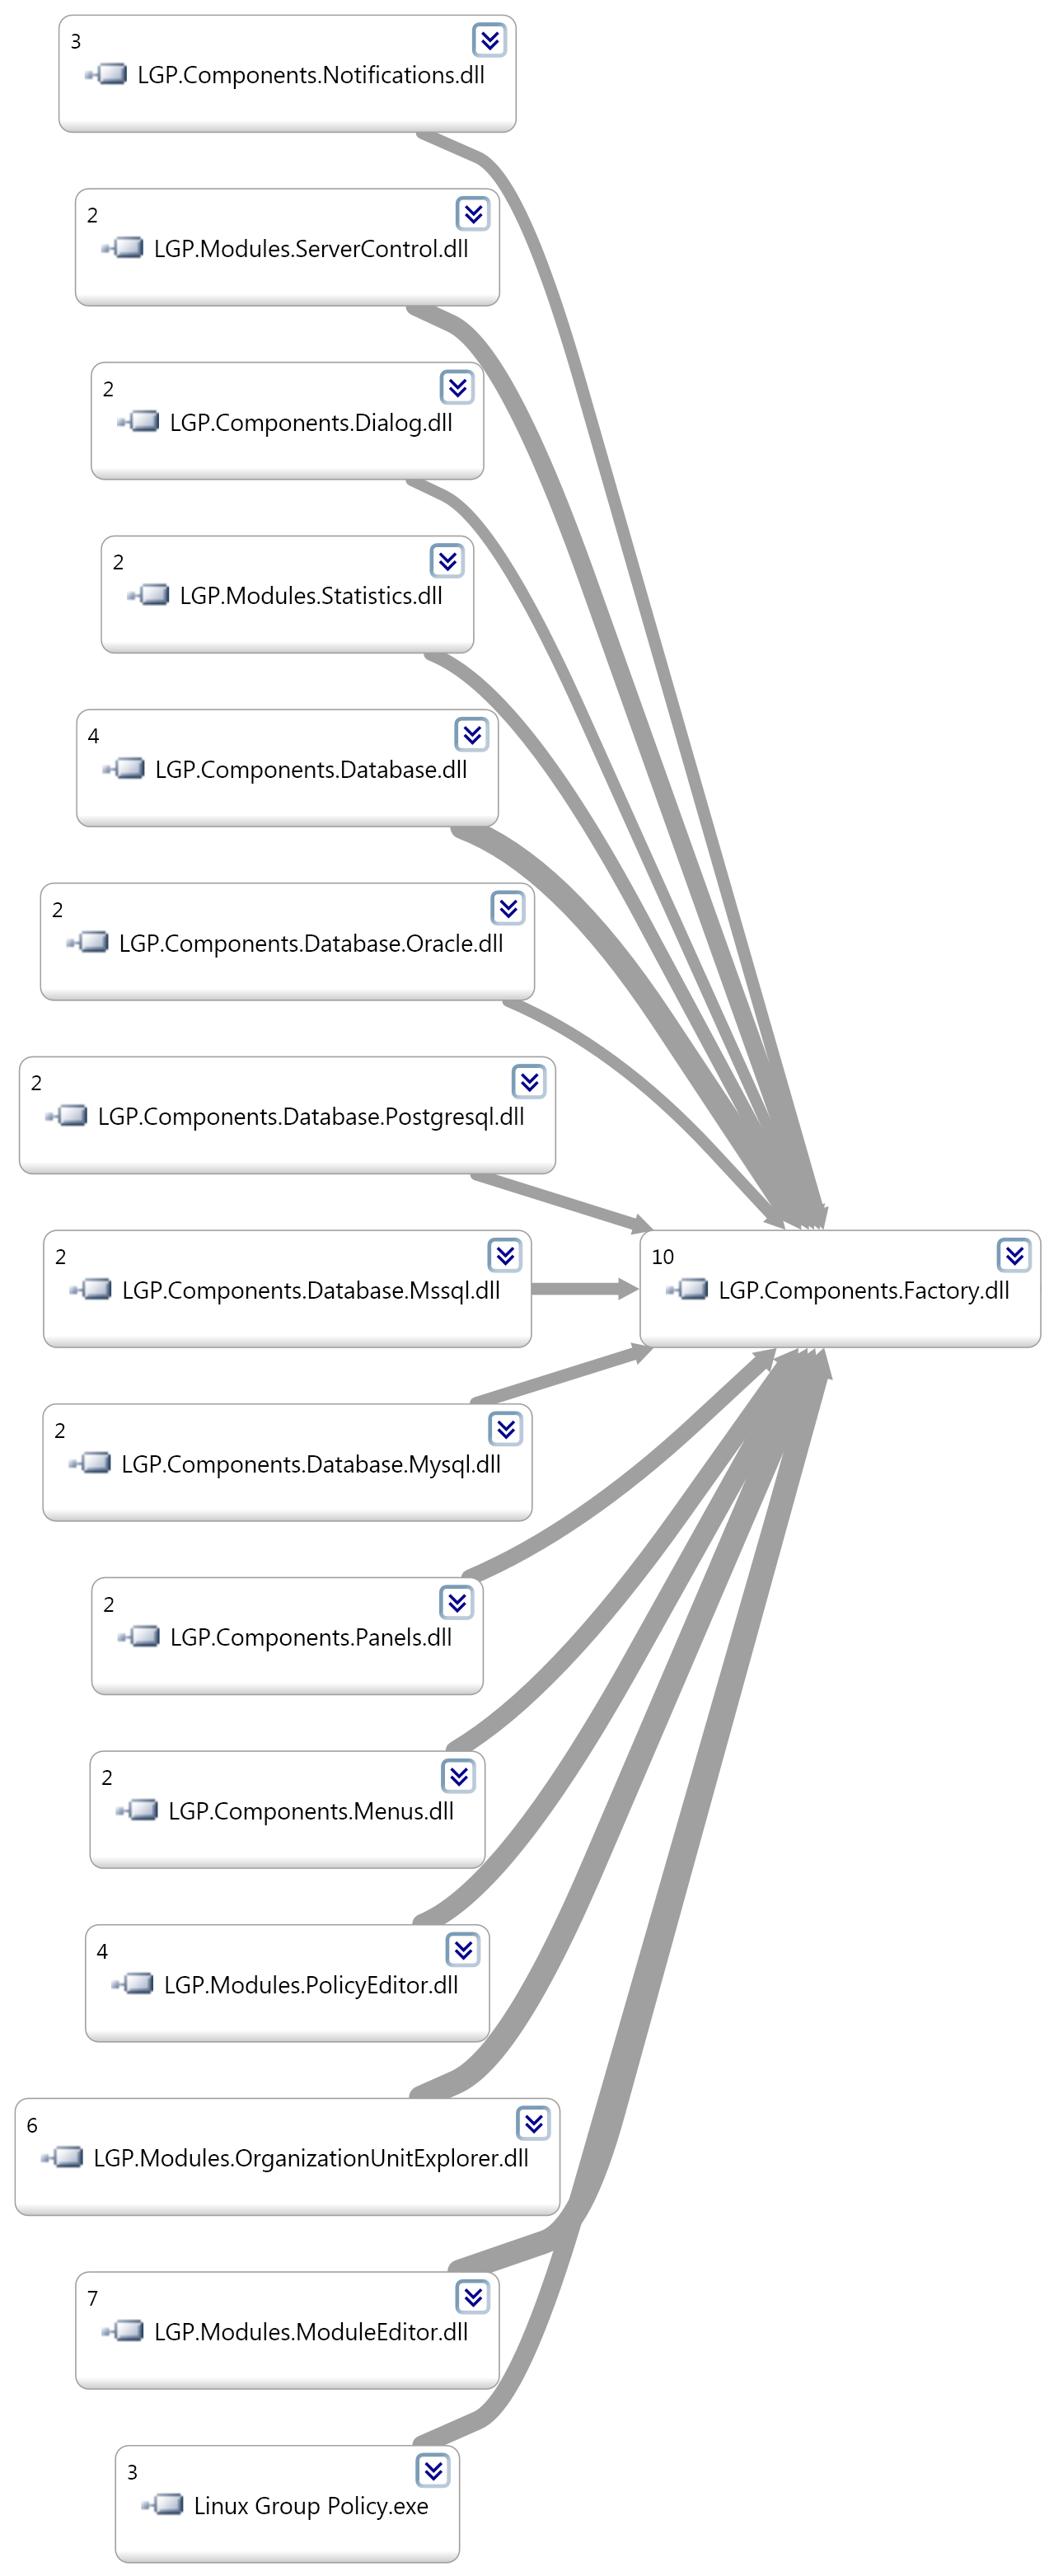
\includegraphics[scale=0.25]{pages/chapter3/figures/archover.png}
				\vspace{-2mm}
				\caption{Composite Architecture Overview}
				\label{fig:archover}
			\end{figurehere}	
		
		\end{multicols}
		
\newpage
				
		\normalsize
		{			
			This reduces the coupling and in effect the modules are not dependent on any one particular 
			concrete type other than that of the Framework boundary class.  The framework class exposes either directly or indirectly 38 separate interfaces 
			consisting of domain specific and non domain specific interfaces.  
			An excerpt of the framework class's auto properties (gets/sets) can be seen in Fig. \ref{fig:FrameworkClass}
			\newline
		}
		
		\indent\begin{minipage}{\textwidth}
			
			\begin{center}
			\begin{figurehere}
				\centering
				\inputminted[linenos=true,fontsize=\footnotesize,tabsize=2]{csharp}{pages/chapter3/smippets/framework.cs}
				\vspace{-5mm}
				\caption{Framework Static Class}
				\label{fig:FrameworkClass}
			\end{figurehere}	
			\end{center}
		
		\end{minipage}
			
		\vspace{5mm}	
		\normalsize
		{
			Where certain modular interaction is required the framework also provides a global uniform support for message passing.  This implementation 
			is based upon Martin Fowler's Event Aggregator design pattern.  This pattern allows publishers and subscribers to evolve independently of one 
			another, furthermore this modular approach to message passing fits well with the overall architectural design.  
			The published events of the event aggregator in the implementation are somewhat generic and therefore limited in application. 
			\newline
			\newline
			For specific interaction, an alternative approach was needed and the identification certain state transitions were identified 
			for exposure within the dynamic link library entity classes.  
			For example, right click context menus in modular systems are populated not only with menu options 
			from the implementing dynamic link library control class, but also the allowance or ability for other dynamic link library classes 
			to inject options into that menu as required.  
			\newline
			\newline
			This menu is generally specific to a type, ie. menu options for inode control 
			(file, directories) would not be applicable to a text editors right click menu.  Therefore differentiation of the specific 
			contexts are needed and in the framework implementation; these contexts are identified by the 38 separate interfaces Fig. \ref{fig:archinterfaces},
			specifically the domain specific interfaces Fig. \ref{fig:domaininterfaces}.  
			For third party developers, it is their choice whether or not to expose these transition states.
		}

		\vspace{3mm}
		\noindent\begin{minipage}{\textwidth}
			
			\begin{figurehere}
				\centering
				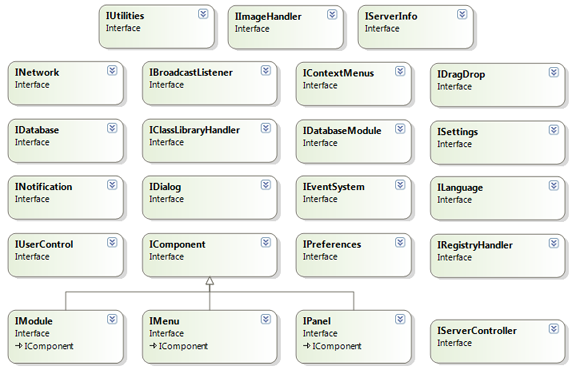
\includegraphics[scale=0.85]{pages/chapter3/figures/factory-interfaces-med.png}
				\caption{Architectural Interfaces}
				\label{fig:archinterfaces}
			\end{figurehere}
		
		\end{minipage}
		
		\vspace{3mm}
		\normalsize
		{
			An example of this within the application can be observed within the Organisational Unit explorer.  The right click menus on an Organisational
			Unit are exposed and the policy editor which is a separate independent module, injects its' ``edit policy'' menu.  The Event Aggregator pattern
			and Context Menu Injection Pattern can be referenced in section \ref{sec:LGPAdminCoding}.
			\newline
		}
							
		\large{\bfseries{Interfaces}}
		\newline		
		\normalsize
		{
			The architectural interfaces in Fig. \ref{fig:archinterfaces} \& \ref{fig:domaininterfaces} are used to decouple the dynamic link libraries from one another.
			These architectural interfaces are focused primarily with the inner workings of the application, the identification of 
			non domains specific classes, such as boundary or control classes concerned with user interface components, database access and networking.  
			\newline
			\newline			
			The following,  IOu, IClient, IGrammer, IPolicy and IModule are the domain specific interfaces.  The gateway interfaces are oriented around the
			Martin Fowlers' Table Gateway Pattern discussed later in this section, the subsequent observers and the separation of these interfaces.			
		}
			
		\noindent\begin{minipage}{\textwidth}
			
			\begin{figurehere}
				\centering
				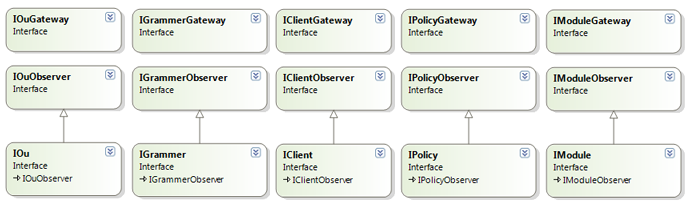
\includegraphics[scale=0.65]{pages/chapter3/figures/domainspecificinterfaces.png}
				\caption{Domain Specific Interfaces}
				\label{fig:domaininterfaces}
			\end{figurehere}
		
		\end{minipage}		
	
	\subsection{Patterns}
	
		\normalsize
		{	
			A key concern of any database centric product is the validity of the data.
			Dirty data in a database can lead to problems, for migrations and upgrades.  Research into the area revealed that many approaches to 
			controlling database access have been maturely established.  Many patterns were considered before implementation occurred. 
			Some of the design patterns considered where Query Object, Record Set, Row Data Gateway, Single Table Inheritance, Table Data Gateway, Table Module,
			Gateway, Active Record, Association Table mapping, Class Table Inheritance, Concrete Table Inheritance, Data Mapper and Data Session State to name a few.
			After careful consideration of uses cases, a modification of Table Data Gateway and Row Data Gateway was chosen. 
			\newline
		}
		
		\large{\bfseries{Table Data Gateway}}	
		\newline		
		\normalsize
		{			
			Table Data Gateway was an obvious candidate for manipulating a database table as a whole, from Patterns of Enterprise Application Architecture,
			Martin Fowler describes it as \emph{ "An object that acts as a gateway to a database table. One instance handles all rows in the table"  }	
			- \citet{FowlerPatternsArchiteture}. Simply put the Table Data Gateway is more like a collection data structure (list, arraylist, linkedlist), 
			smarts bits can be implemented to control or buffer the data too and from the database.
			\newline
			\newline
			This gateway implements methods similar to that found in the aforementioned collection types.  For example an Employee gateway
			would implement methods such as, get, add, remove and search.  These methods encapsulate the SQL ( structured query language ) statements
			that are used to query the database.  This abstracts database interaction from the plugin developers and reduces / negates the possibility of
			poorly constructed queries that may cause inefficient queries or in some cases harmful queries.  The following sample is used in the implementation
			as a control class for accessing the organisational unit table.
		}
			
		\vspace{2mm}
		\begin{figurehere}
			\inputminted[linenos=true,fontsize=\footnotesize,tabsize=2]{csharp}{pages/chapter3/smippets/ougateway}
			\vspace{-2mm}
			\caption{Organisational Unit Table Gateway}
			\label{fig:ougateway}
		\end{figurehere}

\newpage		
		
		\large{\bfseries{Row Data Gateway}}
		\newline
		\normalsize
		{
			\label{sec:RowDataGateway}
			On inspection of the interface in Fig. \ref{fig:ougateway} another type is recognised, ``Iou''.  This brings us to the second pattern Row Data Gateway
			and from Patterns of Enterprise Application Architecture, Martin Fowler describes it as \emph{ 
			"An object that acts as a gateway to a single record in a data source. There is one instance per row" } - \citet{FowlerPatternsArchiteture}.  
			As previously stated the Table Gateway can be described as a collection class and as a result Row Data Gateway complements this pattern.  
			\newline
			\newline
			Each row in the table is to be represented as an object in the system, to be encapsulated by the collection class.  
			Each column field within that row is a property of this object which needs to be encapsulated and appropriate rules or business logic embedded
			into accessors and mutators of this object.  This adds a second layer of data checking and enforcement of constraints to the data.  This second layer
			of perplexity ensures the reduction of dirty data in the tables. A database generally achieves this via foreign key constraints within the database.  
			However for fields in the database where constraints cannot be determined or accurately implemented via the internal data restriction mechanisms,
			the mutators of the object representation offer an area to ensure the validity of the data before updating the database.	
		}
		
		\vspace{5mm}
		\begin{figurehere}
			\inputminted[linenos=true,fontsize=\footnotesize,tabsize=2]{csharp}{pages/chapter3/smippets/ou}
			\vspace{-2mm}
			\caption{Organisational Unit Row Gateway}
			\label{fig:ou}
		\end{figurehere}
					
		\vspace{5mm}
		\normalsize
		{
			These two patterns in conjunction have many implementation concerns, such as the where and how updates are done.
			In this proof of concept implementation i decided to reduce the complexity and separate the concerns.  As such the 
			Table Gateway is concerned with managing the collection, and the row gateway is concerned with modifying its represented row.
			\newline
			\newline
			Developers may choose to use generics; also know as templates in C++, to implement generic gateways to be instantiated
			with specific types at run time.  This is an implementation concern that serves promote the re-usability of these gateways, however
			at the possible cost of security and control of the data, it was not decided to go this direction.
			\newline
		}	
		
\newpage
	
		\large{\bfseries{Event Aggregator}}
		
		\normalsize
		{
			The Event Aggregator design pattern by Martin Fowler is a publish subscribe design pattern.  Events are published 
			and subscribed to by means of an event handler control class.  This control class provides access to concrete implementations
			of composite presentation events which acts a broker for type based messages.
			\newline
			\newline
			Typical implementations of this pattern approach it in this manner, for the separation of event types.  
			The reason for this approach is that in large systems with many publishers and subscribers, the iteration of all the subscribers 
			for a published message, can be expensive.  Therefore the separation of the events and their composition event control classes is preferred.
			Fig. \ref{fig:EventAggregatorTypeBased} shows a high level overview of this approach.
			\newline
		}
		
		\begin{figurehere}
			\centering
			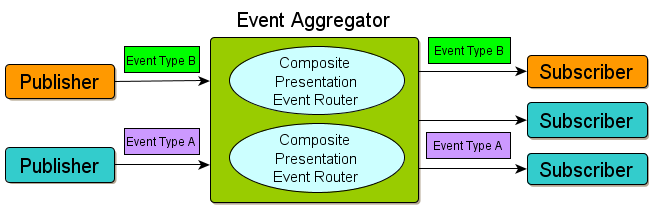
\includegraphics[scale=0.68]{pages/chapter3/figures/ean.png}
			\caption{Event Aggregator - type based}
			\label{fig:EventAggregatorTypeBased}
		\end{figurehere}
		
		\vspace{5mm}
		\normalsize
		{
			For a large architecture, this is the ideal approach for the best performance, security and decoupling concerns.
			However in the project these concerns did not out way the overhead of the separation of events, their handlers, their interfaces
			and the overall increase of types and resulting coupling within the system.  Therefore I decided to use a generics approach.
			By creating a generic composite presentation event router and with the use of domain interfaces this explosion of types
			was negated.  I left it up to the subscriber to determine whether the message that was received was of the type it was concerned with.
			This moved the responsibility of the type interpretation from the event router to the event receiver.	Fig. \label{fig:EventAggregatorGenericBased}
			presents this generics approach.
			\newline
		}
		
		\begin{figurehere}
			\centering
			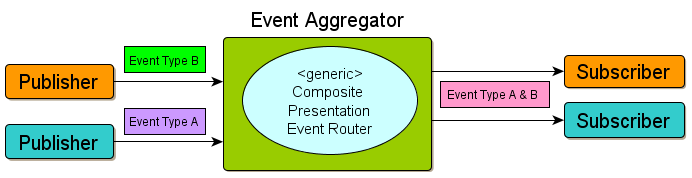
\includegraphics[scale=0.62]{pages/chapter3/figures/eag.png}
			\caption{Event Aggregator - generic based}
			\label{fig:EventAggregatorGenericBased}
		\end{figurehere}
		
\newpage
	
	\subsection{Coding} 
		\label{sec:LGPAdminCoding}
			
			
		\normalsize
		{		
			Unlike the relatively simplistic flexibility of interpreted languages, the implementation of the presentation user interface required
			greater knowledge.  A deep understanding of the concepts of binding, dynamic dispatch and reflection had to be well understood in order
			to create the composite architecture.
			The knowledge base required was not limited to these fundamental or computer science software characteristics.
			An understanding of user interface design and concepts such as routed events and event bubbling was mandatory.
			\newline
			\newline
			In this section i will attempt to articulate these concepts, as they were used in the software architecture developed.
			\newline
		}
		
		\large{\bfseries{Reflection and the loading of composites}}
		\newline
		\normalsize
		{
			As previously discussed in the architectural overview, the composite approach is achieved via the use of reflection.  
			Reflection is a process by which a computer program can inspect a type at run time.  It is not limited to just inspection,
			as it can be used to modify an objects structure and behavior at run time.  In the architectural design however, reflection is 
			primarily used for inspection of the of composites and their internal types.  These types that match, support, realise architectural interfaces
			are loaded and referenced in the appropriate location.  These objects are then exposed via the Framework static class as previously discussed.
			\newline
			\newline
			Fig. \ref{fig:reflection} presents an example of the use of reflection.  In this example a composite or assembly is loaded and
			through this assembly reference, the inspection of it's internal types is done.
			The goal in this example, is the search for a type that realises the IContextMenus interface.  When it is found, it is assigned to 
			an internal member property, which can then be later accessed via an accessor (GET method).
			\newline
		}
		
		\begin{figurehere}
			\inputminted[linenos=true,fontsize=\footnotesize,tabsize=2]{csharp}{pages/chapter3/smippets/reflection}
			\caption{Using reflection to load modules}
			\label{fig:reflection}
		\end{figurehere}
		
		
		
		
		\large{\bfseries{Exposing of these loaded types}}
		\newline
		\normalsize
		{
			As seen here in Fig. \ref{fig:reflection} which is an excerpt of the ClassLibraryHandler class, a class that realises
			this IContextMenus is loaded and exposed.  To put this in context, Fig. \ref{fig:framework} shows the exposure of this 
			type via the Framework static class.  The type exposed is the interface and not the concrete type, therefore this effectively decouples 
			other composites from the concrete implementation of said type.  In order to make use of this functionality, other composites
			include a reference to the Framework static class.
		}

		\vspace{5mm}
		\begin{figurehere}
			\inputminted[linenos=true,fontsize=\footnotesize,tabsize=2]{csharp}{pages/chapter3/smippets/framework}
			\vspace{-5mm}
			\caption{Framework exposing plug-ins via interfaces}
			\label{fig:framework}
		\end{figurehere}
		
		
		
		
		
				
		\vspace{3mm}
		\large{\bfseries{IContextMenus}}
		\newline
		\normalsize
		{	
			Following on from the loading and exposing of this type, Fig. \ref{fig:IContextMenusinterface} depicts the method signatures of this interface.
			This interface provides access to the architectural support, for registering of menu items, in context menus dynamically at run time.  
		}
				
		\vspace{4mm}
		\begin{figurehere}
			\inputminted[linenos=true,fontsize=\footnotesize,tabsize=2]{csharp}{pages/chapter3/smippets/IContextMenus.cs}
			\vspace{-5mm}
			\caption{IContextMenus interface}
			\label{fig:IContextMenusinterface}
		\end{figurehere}
		
		
		
		
		
		
		\vspace{3mm}
		\normalsize
		{		
			The RegisterContextMenuItem allows plug-ins to register menu items to be dynamically embedded into a context menu.  The three parameters 
			specify the type that will be passed back to the registering handler, the menu item which will physically be displayed in the context menu and 
			finally the Action, which is a delegate for an encapsulated callback method.
			\newline
			\newline
			In Figure \ref{fig:registration} plugin A registers menu items with the context menus handler (IContextMenus).
			The callback method, the final destination of the menu item click is where the ITargetItem is sent. 
			\newline
		}
			
		\vspace{-2mm}
		\begin{figurehere}
			\inputminted[linenos=true,fontsize=\footnotesize,tabsize=2]{csharp }{pages/chapter3/smippets/registerMenuItem}
			\caption{Plugin A : Register menu item with the framework}
			\label{fig:registration}
		\end{figurehere}
			
		\vspace{3mm}
		\normalsize
		{
			In Figure \ref{fig:attachregistration} plugin B accepts menu registrations for ItargetType and requests the 
			context menus handler (IContextMenus) to append them to the context menu. The menu item click handles the actual click event.
			This allows ``smart bits'' to occur before asking the context menus handler (IContextMenus) to invoke the CallBackMethod in plugin A.
			This decouples the plug-ins from one another, coupling the two with IContextMenus and any ``Type'' in this instance ITargetType.
			\newline
		}	
					
			
		\begin{figurehere}
			\inputminted[linenos=true,fontsize=\footnotesize,tabsize=2]{csharp}{pages/chapter3/smippets/contextOpeningEvent}
			\vspace{-2mm}
			\caption{Plugin B : Handle menu item click and invoke callback}
			\label{fig:attachregistration}
		\end{figurehere}			
			

		
		

		\vspace{3mm}
		\large{\bfseries{Dynamic Context Menus Sequence Diagram}}
		\newline
		
		\begin{figurehere}
			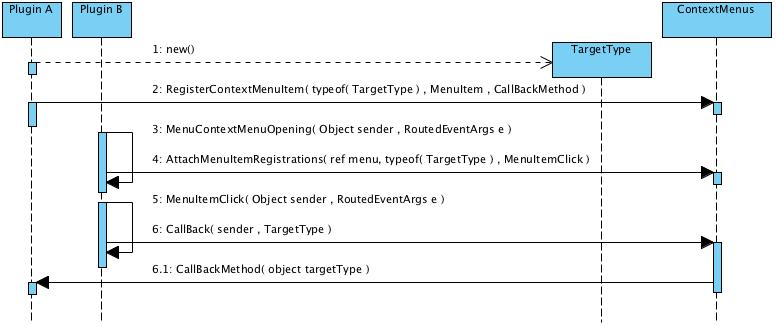
\includegraphics[scale=0.6]{pages/chapter3/figures/SequenceContextMenus2.jpg}
			\caption{Context Menus hooks sequence diagram}
		\end{figurehere}
						

\newpage
						

	\subsection{Analysis}
	
		\normalsize
		{	
			A widely accepted concept in software design is the decoupling of components(composites) or the minimisation of inter dependencies, to promote re-usability.  
			There are many papers that target interface definition as the means to accomplish this, such as, 
			``A comprehensive interface definition framework for software components'' \& ``An Approach to Software Component Specification'' by \citet{JunHan}.
			With this software paradigm preposition, I am going take a look at the more fundamental concern of component (composite) based design. 
			\newline
			\newline
			David Lloyd of JGroup Expert defines the distinction between libraries and frameworks :
		}	
			
		\vspace{-5mm}
		\begin{multicols}{2}
		
			\begin{itemize}		
				
				\item \textit{\textbf{Library}}	
				
					\begin{itemize}
			
						\item \textit{Set of classes instantiated by client}							
						\item \textit{Client calls functions}		
						\item \textit{No predefined flow of control}
						\item \textit{No predefined interaction}
						\item \textit{No default behaviour}						
					
					\end{itemize}
				

		\columnbreak
					
				\item \textit{\textbf{Framework}}	

					\begin{itemize}
			
						\item \textit{Customisation by sub-classing}							
						\item \textit{Calls client functions}	
						\item \textit{Controls flow of execution}							
						\item \textit{Defines object interaction}	
						\item \textit{Provides default behaviour}	
					
					\end{itemize}
					
			\end{itemize}

		\end{multicols}
		
		\vspace{-2mm}
		\normalsize
		{		
			Given the aforementioned premises of architectural design goals and the distinction between libraries and frameworks; 
			it may seem that libraries do not exhibit characteristics prevalent to achieve decoupled components (composites).  The instantiation
			of classes and calling of functions directly, couples components (composites).
			\newline
			\newline		
			Composite design therefore even with good interfaces and supporting factory methods still presents coupling.  This coupling as stated comes in the form 
			of factory methods that require access to one or more concrete types in a composite.  If there are multiple interdependencies between composites
			changing out a composite may present difficultly in the form of refactoring.
			\newline
			\newline
			The fundamental concern is then composite interdependencies.  The characteristics of a framework provide greater composite decoupling.  
			The presentation framework for the admin interface provides only one concrete dependency relationship, targeting this concern.		
			The admin presentation interface evolved to the characteristics of a framework, which I believe is a bigger concern, than good interface
			definition.  This concept comparable to networking is the difference between a mesh network and a star network, as seen in Fig. \ref{fig:Interdependance}.
			\newline
		}
		
		\begin{figurehere}
			\centering
			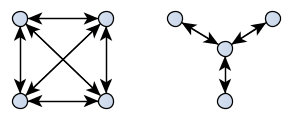
\includegraphics[scale=1.0]{pages/chapter3/figures/interdependance.png}
			\caption{Interdependence - Mesh(L) - Star(R)}
			\label{fig:Interdependance}
		\end{figurehere}
	
\newpage	
	
	\subsection{Improvements}

		There are many advantages and disadvantages to the framework developed.  The architectural framework devised is rigid in many respects.  
		As all classes in the factory composite are defined as ``internal'' classes and exposed via their interfaces, this does not offer any sub-classing 
		and changing of behaviour to composite developers.  This effectively locks developers into the behaviour of the architectural framework.
		\newline
		\newline
		To address this concern, firstly the reasoning for this approach must first be addressed.  During coding it is common practice to exercise encapsulation
		when implementing classes and through the use of accessors and mutators, this basic object oriented principle is adhered to.  Similarly when designing composites
		this practice can be achieved via ``internal'' classes.  This effectively means that peer composites cannot instantiate these classes marked as internal.
		\newline
		\newline
		For future improvements to the architectural framework, a relaxing of this principle may be applied.  Classes that are not deemed critical to core
		functionality or do not present a security concern, may be marked as public.  Alternatively patterns to support other functionality or
		out of band services would be the preferred approach.  An analysis of composite developer requirements should be completed and patterns implemented in 
		future revisions to support these requirements.
		
		

	
	\newpage

\section{Database} 

	\subsection{Requirements}
	
		\normalsize
		{		
			\begin{enumerate}[itemsep=1pt,parsep=1pt]
				\item Storage of rules
				\item Common non ambiguous names for rules
				\item Organisational Units and Clients
				\item Globally unique identifiers (GUID) for computer objects. 
			\end{enumerate} 		
		}
	
	\subsection{Design}	

		\normalsize
		{
			The design of the database was minimalist given the requirements.
			Fig. \ref{fig:dbdesignoverview} presents the relational design and
			abstraction of the domain concepts.  As seen in presentation admin 
			interface these entities are represented by design patterns.
			The main requirements are satisfied, ``policy'' table for the storage of rules,
			and the representation of clients and organisational units. 	
			\newline			
		}
	
		\begin{figurehere}
			\begin{center}
			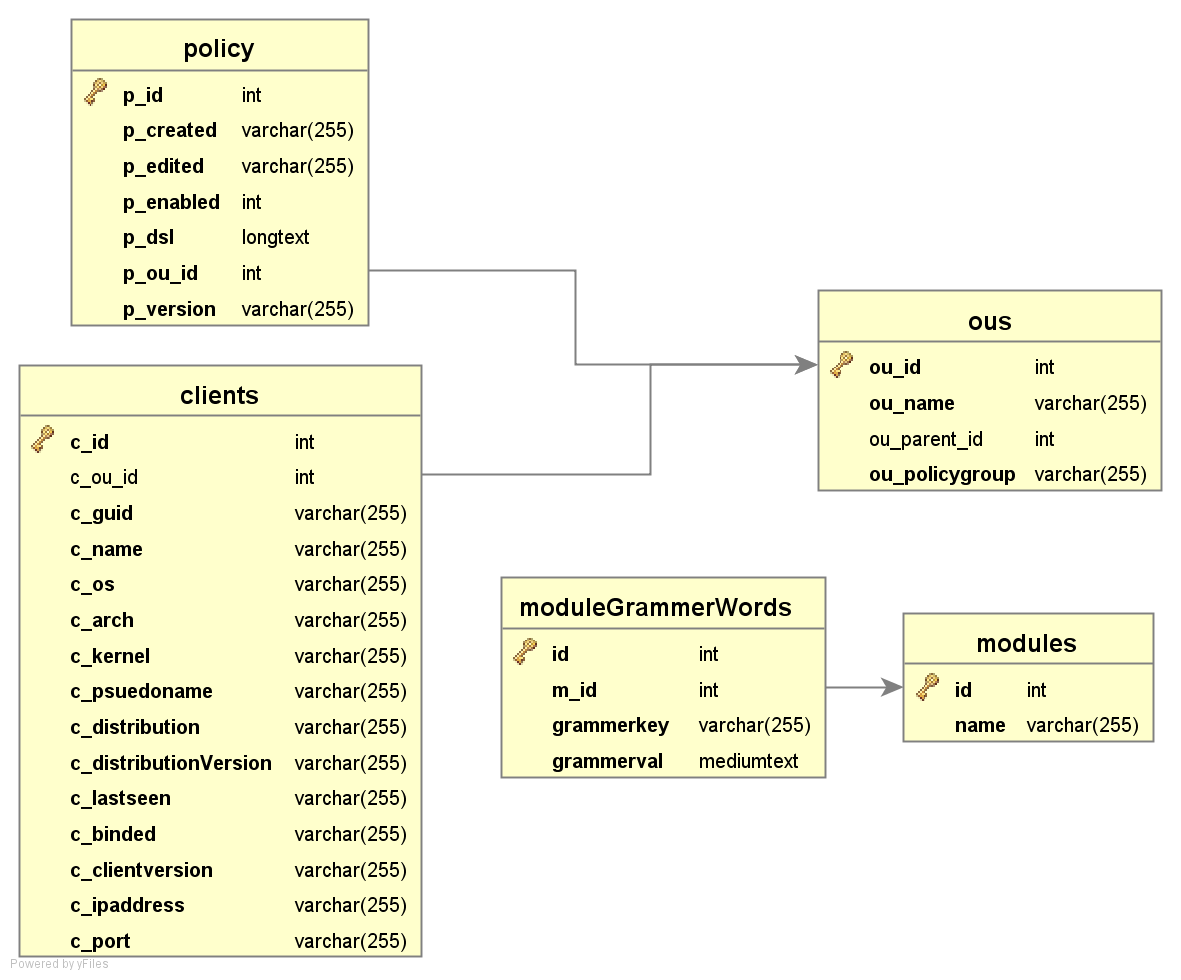
\includegraphics[scale=0.35]{pages/chapter3/figures/db.png}
			\end{center}
			\caption{Database Design Overview}
			\label{fig:dbdesignoverview}
		\end{figurehere}	
	
	\subsection{Analysis \& Improvements}
	
		\normalsize
		{
			Without an analysis of component developer requirements and future development, it's hard to say what improvement would be made to the database design.
			An obvious choice we be the adjustments of the types.  There is extensive used of varchar, however as the data
			is used primarily as strings within the application for display purposes, this may not be necessary.
		}
	

	
	\newpage

\section{Domain Specific Language} 
\label{sec:Domainspecificlanguage}

	A Domain Specific Language in many circles is generally described as a computer programming language with limited expressiveness,
	focused on a particular domain.  The best example of this description is the hypertext markup language (HTML) and
	of course everyone's favourite the structured query language(SQL).
	\newline
	\newline
	Domain specific languages are not a new concept.  
	The structured query language(SQL) was conceived 1986 \& the hypertext markup language (HTML) 1989.
	The choice for a Domain Specific Language (DSL) depends largely on what you are trying to achieve and whether this
	succinct language offers more efficient, less verbose and more flexibility; but even more so, is it better suited for the domain.
	Would it be efficient for people to do database queries in the Extensible Markup Language (XML)?   For those who are familiar with
	oracle's structured query language(SQL) command line interface, imagine using it with the Extensible Markup Language (XML).
	\newline
	\newline
	Moving quickly on from this eye brow raising statement, the choice for a Domain Specific Language in the solution was evident.
	Having experience in other solutions, such as INI files, Javascript Object Notation (JSON) and Extensible Markup Language (XML);
	these seemed rather verbose and restrictive to administrators who wished to define rules quickly and cleanly.
	Language cacophony is a common objection to taking on a Domain Specific Language (DSL).  However this argument is quickly avoided
	by the purpose of the Domain Specific Language (DSL).  The purpose of the Domain Specific Language (DSL) is to reduce the complexity of the statements
	used to achieve a domain specific goal.  Writing a web site in Java would be quiet a difficult and time consuming task; 
	this is why hypertext markup language (HTML) was conceived.
	\newline
	\newline
	As PERL was used as the client side implementation, this offered the perfect solution for text processing and the foundation for a Domain Specific Language (DSL).
	PERL, the practical extraction and reporting language was developed for text processing.  PERL has many tools for this activity, one of them being Filters.
	Filters or pre-processing of an input file, allowed for the formulation of this conceptual requirement.  As pre-processing can analyse the domain specific
	language, post-processing can also execute internal or embedded PERL statements, giving rise to the concept of a hybrid Domain Specific Language (DSL).
	\newline
	\newline
	Stepping back from this assertion for the moment, what is the difference between an ``internal'' and an ``external'' Domain Specific Language (DSL)?
	To be short and succinct in the definition of these two terms, an internal Domain Specific Language (DSL) is code that can be evaluated and executed
	without syntax directed translation taking place, to achieve the native language understood by the parser; while an external Domain Specific Language (DSL) is code
	that requires some sort of translation before it is understood by the parser.
	\newline
	\newline
	The following sections will identify these concepts in the implementation.
	
\newpage	

	\subsection{Requirements}
	
		\normalsize
		{
			\begin{enumerate}[itemsep=1pt,parsep=1pt]
				\item 	An extensible Domain Specific Language.
				\item 	Domain Specific Language grammar hooks.
				\item 	Hybrid Domain Specific Language.
				\begin{itemize}
					\item Internal characteristics, rules provided by modules.
					\item External characteristics, embedded PERL.
				\end{itemize}
			\end{enumerate} 		
		}
	
	\subsection{Design}
	
		\normalsize
		{
			The design of the Domain Specific Language (DSL) is based primarily on the extensibility of the client interpreter.  In previous
			sections we looked at how new parsing rules were injected into the interpreter.  These rules essentially define the Domain Specific Language (DSL).
			Therefore the language is not restricted by a document type definition (syntax and ordering rules).
			This means that the Domain Specific Language (DSL) constantly changes as interpreter modules are created and edited.
			Therefore the design of the Domain Specific Language (DSL) is the sole responsibility of the PERL module developers.
			\newline
			\newline
			Fig. \ref{fig:DSLHybrid} shows both examples of the internal \& external Domain Specific Language (DSL) statements.
			The internal Domain Specific Language (DSL) statements are identified between the \% symbols.
			An example of an external Domain Specific Language (DSL) statement, namely ``SERVICE\_CONTROL'' will be parsed by the rules
			provided by an interpreter module.
		}
		
		\vspace{2mm}
		\begin{figurehere}
			\inputminted[linenos=true,fontsize=\footnotesize,tabsize=2]{perl}{pages/chapter3/smippets/dsl2}
			\vspace{-5mm}
			\caption{DSL - Hybrid}
			\label{fig:DSLHybrid}
		\end{figurehere}	
		
		\vspace{2mm}
		\normalsize
		{
			Parsing of the internal statements is quiet simple and articulated in Fig. \ref{fig:InternalParsing},
			while the parsing of the external statements is shown in Fig. \ref{fig:ExternalParsing}
		}
		
		\vspace{2mm}
		\begin{figurehere}
			\inputminted[linenos=true,fontsize=\footnotesize,tabsize=2]{perl}{pages/chapter3/smippets/pe.txt}
			\vspace{-5mm}
			\caption{DSL - External Parsing}
			\label{fig:ExternalParsing}
		\end{figurehere}

\newpage		

		\vspace{4mm}
		\begin{figurehere}
			\inputminted[linenos=true,fontsize=\footnotesize,tabsize=2]{perl}{pages/chapter3/smippets/pi.txt}
			\vspace{-5mm}
			\caption{DSL - Internal Parsing}
			\label{fig:InternalParsing}
		\end{figurehere}			
	
	\subsection{Analysis \& Improvements}
	
		\normalsize
		{
			The hybrid characteristics of the Domain Specific Language (DSL) offers the greatest possible flexibility for administrators.
			By allowing the embedment of PERL into the Domain Specific Language (DSL), administrators who are waiting for new additional functionality to be provided 
			by me the developer, can work around any deficiencies discovered within the implementation.
		}
	
\newpage
	

	
	\newpage

\section{Supporting Technologies}
				
	\normalsize
	{			
				
		\begin{itemize}
					
			\item \textbf{Gentoo Linux}
				\newline						
				Gentoo a distribution of Linux is built on top of the portage package management system.  
				The system is compiled directly from source and allows the user to choose the features or compile options when building their system.
							
			\item \textbf{Ubuntu Linux}	
				\newline								
				The Ubuntu distribution is a fork of the Debian Linux operating system.  The design philosophy of
				this distribution is geared towards usability and the desktop experience and therefore for home personal use.
				
			\item \textbf{Opensuse Linux}	
				\newline								
				Open use is the free version of Novell's Suse Linux Enterprise Server.  The design of Suse is about constant refinement as opposed to 
				bleeding edge software.  As such its considered one of the mature Linux operating systems.
				
			\item \textbf{Redhat Linux}		
				\newline							
				Red Hat the largest corporate contributor to the Linux kernel, provides Enterprise Linux and open-source enterprise 
				middle ware solutions such as JBoss. Red hat provides operating-system platforms 
				along with middle ware, applications, and management products, as well as support, training, and consulting services.
				Red Hat creates, maintains, and contributes to many free software projects.
				
			\item \textbf{Fedora Linux}	
				\newline								
				Fedora sponsored by Red Hat is mainly driven towards the promotion and advancement leading edge of open source technologies
				
			\item \textbf{CentOs Linux}	
				\newline								
				CentOs is the licence free downstream version of the Red Hat Enterprise Linux operating system.
						
			\item \textbf{VmWare Workstation}	
				\newline								
				Vmware Workstation, Vmware flagship consumer product is the desktop solution for Virtual Operating Systems.
				This product allows for multiple virtual machines to be hosted on a single computer.
				
			\item \textbf{VmWare Workstation}	
				\newline								
				Vmware Workstation, Vmware flagship consumer product is the desktop solution for Virtual Operating Systems.
				This product allows for multiple virtual machines to be hosted on a single computer.
				
			\item \textbf{Visual Paradigm}	
				\newline								
				Visual Paradigm was used for some of the unified modelling language diagrams
				
			\item \textbf{Subversion}	
				\newline								
				Subversion was used as the primary source version control.	

		\end{itemize}
		
	}

\newpage

		

	


	
	
	